\documentclass[12pt,twoside]{report}
\usepackage[utf8]{inputenc}
\usepackage[english]{babel}
\usepackage{polski}

\usepackage{graphicx}
\usepackage{float}
\usepackage{xcolor}
\usepackage{wrapfig}


\usepackage{textcomp}
\usepackage{amsmath}
	\numberwithin{equation}{subsection}
\usepackage{caption}
\usepackage{subcaption}

\setlength\parindent{0pt}
\usepackage{sectsty,textcase}
\allsectionsfont{\MakeTextUppercase}


\usepackage[a4paper,width=150mm,top=25mm,bottom=25mm,bindingoffset=6mm]{geometry}
\usepackage[english]{babel}
\usepackage[nottoc]{tocbibind}
%%%%%%%%%%%%%%%%%%%%%%%%%%%%%%%%%%%%%%%%%
%TABLE OF CONTENTS LETTERS CHANGE
\usepackage{regexpatch}
\makeatletter
\xpatchcmd*{\@sect}{\fi#7}{\fi\@nameuse{format#1}{#7}}{}{}
%%% for sections and subsections we want uppercase
\protected\def\formatsection{\MakeUppercase}
\protected\def\formatsubsection{\MakeUppercase}

%%% the other titles are left unchanged
\let\formatsubsubsection\@firstofone
\let\formatparagraph\@firstofone
\let\formatsubparagraph\@firstofone

%%% the following is necessary only if hyperref is used
\AtBeginDocument{%
  \pdfstringdefDisableCommands{%
    \let\formatsection\@firstofone
    \let\formatsubsection\@firstofone
  }%
}
\makeatother
%%%%%%%%%%%%%%%%%%%%%%%%%%%%%%%%%%%%%%%%%%%%%%%%%
\usepackage{hyperref}

 
\urlstyle{same}

\usepackage{fancyhdr}
	\pagestyle{fancy}
	\setlength{\headheight}{28pt}
	\fancyhead{}
	\fancyhead[RO,LE]{Chapter \thechapter}
	\fancyfoot{}
	\fancyfoot[CO,CE]{\thepage}
\usepackage{csquotes}
\usepackage[backend=biber]{biblatex}
\addbibresource{ref.bib}

\begin{document}

\graphicspath{ {images/} }
\begin{titlepage}
   \begin{center}
       \vspace*{1cm}
       
	   
\includegraphics[width=\textwidth]{logopwr.pdf}
	   
	   \vspace*{5cm}
	   
       \textbf{\Huge TYPE III SOLAR CELLS \vspace{0.1cm} BASED ON QUANTUM DOTS}
       
       \vspace{1.5cm}
       
 	   \Large BACHELOR'S THESIS
 	   
       \vfill
       
	   \textbf{Maksymilian Kliczkowski}
       \vspace{0.8cm}
 
       
 
       \small Faculty of Fundamental Problems of Technology\\
       Wroclaw University of Science and Technology\\
       Poland\\
       \today
 
   \end{center}
\end{titlepage}

\newpage
 \begin{center}
       \vspace*{1cm}
       
	   
\includegraphics[width=\textwidth]{logopwr.pdf}
	   
	   \vspace*{5cm}
	   
       \textbf{\Huge TYPE III SOLAR CELLS \vspace{0.1cm} BASED ON QUANTUM DOTS}
       
       \vspace{1.5cm}
 	   
       
	   \Large \textbf{Supervisor: dr hab. inż. Artur Podhorodecki}
       \vspace{1.8cm}
 
       
 
       \small Faculty of Fundamental Problems of Technology, Experimental Physics Cathedral\\
       Wroclaw University of Science and Technology\\
       Poland\\
       \today
 
   \end{center}
\newpage

\begingroup

\let\clearpage\relax
\chapter*{\textbf{ABSTRACT}}

In this thesis the extensive study of possible and surly optimal materials for Quantum Dot Solar Cells (QDSCs) will be provided to the reader. One will have the opportunity to develop a rather current image of the necessary parts in their architecture which will be supported with an abundant description of the important aspects in engineering a photovoltaic device. With an introduction of its kind we will try to convey a basic but sufficient knowledge of standard terms, light with matter interaction, light spectrum analysis, quantum dots description with their behaviour and a photovoltaic device operation theory with certainly needed quantities that one has to find in order to properly describe a solar cell. With the objective of creating a possibly competitive Quantum Dot Sensitized Solar Cell(QDSSC) the description of methods that we used will be included with a related to it characteristics. One will also be able to use this paper as a review of today's development phase and current technological state of the other scientific groups all around the world.  After a successful development of a solar cell, the analysis and comparison will definitely be provided.

\chapter*{STRESZCZENIE}

W tej pracy skupimy się na badaniu możliwych, a także optymalnych materiałów pod ogniwa słoneczne bazujące na kropkach kwantowych. Możliwe będzie wyrobienie sobie obecnego obrazu potrzebnych w ich budowie materiałów oraz zapoznanie się z wyczerpującym opisem projektowania tychże urządzeń. Wraz ze wstępem przedstawione zostaną wystarczające podstawy oddziaływania światła z materią, analizy spektralnej, opisu kropek kwantowych, działania urządzeń fotowoltaicznych, a także oznaczenia używane w pracy. Wraz z celem stworzenia możliwe konkurencyjnego urządzenia pokazany zostanie również opis użytych metod. Dodatkowo, możliwe będzie również traktowanie pracy jako krótki przegląd obecnego rozwoju technologii zwiazanych QDSSC na całym świecie. Po wykonaniu urządzenia przeprowadzona zostanie również analiza i porównanie wyników.

\endgroup

 
\chapter*{DEDICATION}
To my   
\includegraphics[scale=0.03]{turtle}, family and friends...

\chapter*{DECLARATION}


I hereby declare that the present bachelor's thesis was composed by myself and that the work contained herein is my own. I also confirm that I have only used the specified resources. All formulations and concepts taken verbatim or in substance from printed or unprinted material or from the Internet have been cited according to the rules of good
scientific practice and indicated by footnotes or other exact references to the original source.

\vline

\noindent The present thesis has not been submitted to another university for the award of an academic
degree in this form. This thesis has been submitted in printed and electronic form. I hereby
confirm that the content of the digital version is the same as in the printed version.
I understand that the provision of incorrect information may have legal consequences.
\vfill

(Signature)\hfill (Place, Date)
\vspace{8.5cm}


\chapter*{ACKNOWLEDGEMENTS}

I would like to thank all the people that have helped me during the thesis creation process. I am really grateful to my Supervisor for allowing me to work inside the group and for an opened chapter to fill the new information in. Further, I am truly thankful to Mr Maciej Chrzanowski, who have showed me the lab and instructed me with a great amount of technical knowledge, without which the thesis wouldn't have been done. Last but not least, I am indebted to the group of Prof. Popko for making many of the experiments and measurements available. To whom I did not include, thank you!

\tableofcontents
\listoffigures 
\listoftables

\chapter{INTRODUCTION}
We, as a society nowadays, are in constant demand for energy. Although,
even with the development of calculating, conducting and studying it, we
don't really know what the energy is, we are depending on that abstract
quantity. One might probably say that to study physics is to endure to
study energy in its every possible form. There's a brilliant quote from
Bill Bryson that: ``Energy is liberated matter, matter is energy waiting
to happen.'' What might be incredible is that from this strictly
mathematical quantity we can deduct anything. And what's also important
it is as arbitrary as it gets, depending only on one's reference. From
energy we can create few more important quantities such as \emph{power}
P, which is simply the energy provided per unit time, so:

$$E = \int P\left( t \right)dt$$

The energy will be represented in J (Joules) or eV (electron
volt), which directly describes energy of elementary charge
(\(e \approx 1.602*10^{- 19}C)\) in 1V (Volt) potential.

$$1eV = 1.602*10^{- 19}J$$

Power will be then represented in W (Watts) (\(W = \frac{J}{s}\ ).\)

The rise of energy consumption has proven that in the future we will
almost certainly require even more. From Global Energy Perspective paper 
\cite{Insights2019} we can learn that:

\begin{itemize}
\item Global energy demand will begin to reach a plateau at around 2035, despite a strong population expansion and economic growth, thanks to emphasis on renewable sources, more efficient service industries or more efficient industrial regions.
\item The energy demand and economic growth has became ``decoupled'' for the first time in history.
\item Renewable sources will provide more than half the electricity after 2035.
\end{itemize}

\noindent The reader is strongly recommended to take a look at the document.

\noindent With telling that we can produce energy there's a slick trick given with
the phrase. Energy cannot be simply created, it is just converted from
another source - so nothing is ever lost or miraculously made. The
problems we need to struggle with are then being able to obtain as much
energy from the energy source as it is possible. Of course, as
humankind society is governed by money, we need to keep the cost lowest simultaneously. There is plenty of different energy sources, that we have learned of, to receive energy
from. In Figure \ref{fig:ensour} we can see the most vivid ones nowadays. But with
the human demand fulfilment come great damages and soon depleting
resources of many energy sources such as fossil fuels.


\begin{figure}[H]
\centering
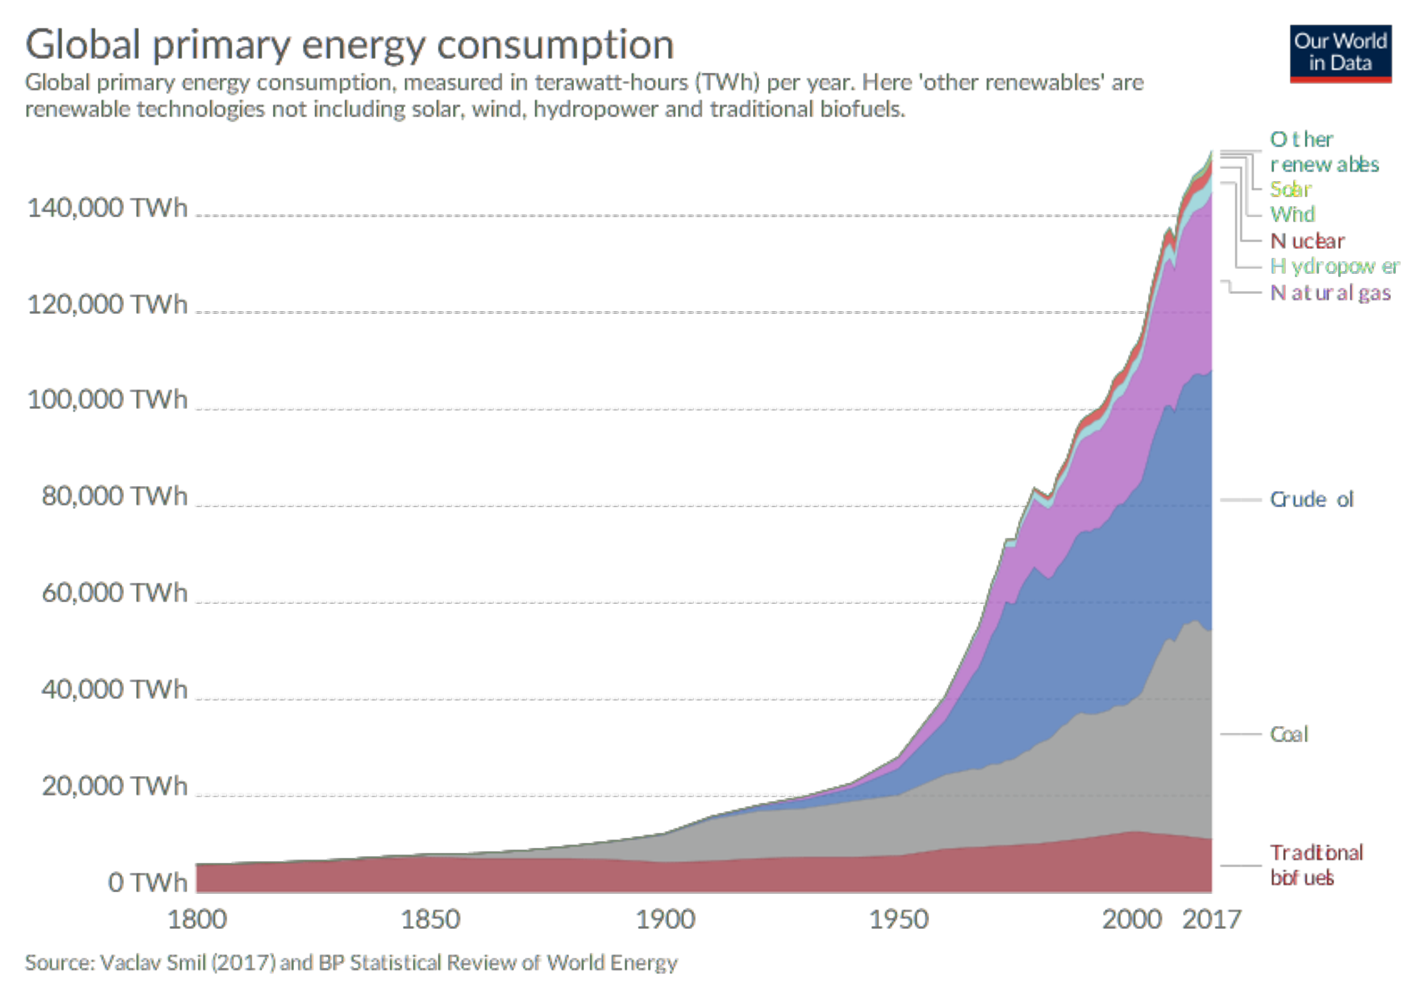
\includegraphics[width=0.6\textwidth]{global-primary-energy}
\caption{Energy sources contribution in world scale
\cite{2019}}
\label{fig:ensour}
\end{figure}

\noindent The necessity of searching new possible ways to harness it through renewable sources has become a global issue. Our concern of the environment had never been that serious before. Not only the change of methods for energy production must be enhanced because of this demand but we need to be strictly aware of the World's urging trepidation of Global Warming, of which evidence is provided for example here \cite{Nasa2019}.

\noindent Among all of the ideas created in a past few decades, solar energy is
believed by many to be one of the most reliable and promising. It can be
directly converted into electricity, heat or chemical energy and our
only Star seems to be an "infinite power" resource for us. In the last ten
years the world solar PV electricity production has grown impressively,
being almost three times bigger in 2016, than in 2010 \cite{2018}. In theory,
the Sun has the potential to fulfil earth's energy demand, if it is not
for the technology. Annually, nearly 10\textsuperscript{18} EJ of energy
reaches our planet and of that 10\textsuperscript{4} EJ is claimed to be
harvest-able. The possibility of converting the solar energy into
electric energy has been studied since discovery of the basic
photovoltaic effect and the development of first semiconductor technologies.

Since the first crystalline silicon solar cell, the technology had undergone a vivid development. The number of different methods that the cell can be created with and the quantity of possible final outcomes isn't inconsiderable. Yet, solar cells can be classified into three generations in accordance to the development technology and materials used\cite{HuashangRao2018}. The first generation describes silicon based solar cells, which so far is the most researched type. It includes mono-crystalline and polycrystalline silicon cells.

The second generation contains thin film solar cells. It refers to amorphous silicon, copper indium gallium selenide (CIGS), GaAs and CdTe devices. With many advantages, such us direct band gaps resulting with harvesting light in very thin films, they still have a small share in the market of PV devices (<10\%) due to their instability and limitation in module technology\cite{HuashangRao2018}.

\begin{figure}[ht]
\label{fig:annual} 
\centering
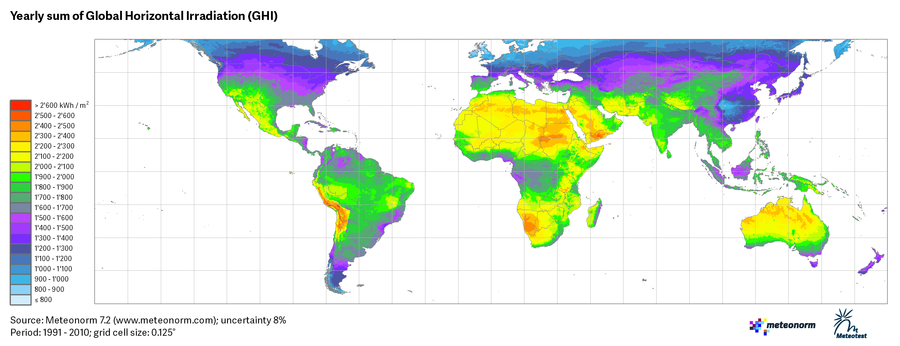
\includegraphics[width=\textwidth]{annual}
\caption{Annual yearly sum of Global Horizontal Irradiation
\cite{1991-2010}}
\end{figure}

The third generation cannot be simplified as much as it's formers. It is usually defined as solar cells that are still in scientific research phase\cite{HuashangRao2018} \cite{GavinCon}. It's main motivation is to achieve a higher efficiency using newly discovered physical phenomena, structures and materials. Their aim shall vary depending on the development technique and the physical principles. Today, the third generation mainly includes perovskite solar cells(PSCs) \cite{PerovRev} \cite{revPerold}, organic/polymer solar cells(OSCs) \cite{Polymer}, dye sensitized solar cells(DSCs)\cite{DyeSent} and quantum dot based solar cells(QDSC). \cite{Kamat2018} While still being considerably less common, the cons of investigating the nature and crucial properties of third generation PVs is overwhelming. Thanks to the ultimate specification of third generation approach, the devices can in perspective generate greater efficiency than other generations(for example by creating multiple electron-hole pairs and multi-band cells), yet while still being significantly cheaper than their formers.

\vline

Our main goal will be to study the QD sensitized solar cells and their characteristics. The base shall be put on PbS quantum dots as a light-harvesting material. We will proceed to consider their tunable band gap and other properties, such as control of composition, dipole moments, stability or collocation, and fit other materials to study the effects and their attributes. In principle, the QD solar cells can be distributed into four different classes: Schottky junction solar cells, p-n junction solar cells, hybrid QD-polymer solar cells and \textbf{quantum dot-sensitized solar cells (QDSCs)} and this is yet to be found later on...

\chapter{Theory}

With this chapter the introduction of some theoretical concepts will be provided. Certainly some of chapters below could be omitted without missing the final result and its meaning. Nevertheless, even if the paper is laced with rather practical analysis and effects, a physicist should be sure to understand the aspects of an experiment well, not just to have a better insight into the outcome but also to be sure that during the process no foolish mistakes are made and to be able to find new methods to improve the research. Therefore, few parts will just be a reminder and introduction to notation used or to ensure the understanding and some will be treated as an inquiry of what might be searched to describe it further. 
\section{Classical and semi classical theory of light and light with matter interaction}
As in the photovoltaic physics we are constantly struggling with the light itself, we should know what the light actually is and how it interacts with matter in many, rather curious and different ways. Why is that so that matter looks the way it does and what of its properties can we control? In this chapter we will embrace the phenomena just to create an image of what we are dealing with. 

\subsection{ELECTROMAGNETIC FIELD}

Before we actually begin we need to state some classic information about
the physics of electric charges. The electromagnetic field is
represented by two, generally complex, vectors, even though the physical
result that we are expecting is ought to be real. Those vectors are
\textbf{E} -- \emph{electric field} and \textbf{B} -- \emph{magnetic
induction}. The properties of those fields are of course described by
the \emph{Maxwell's equations}. For them we shall also introduce two
more important quantities \(\rho\) -- \emph{the electric charge} density
and \textbf{j} -- \emph{electric current density} vector.
We can define them in this way:
\begin{equation}
e = \int\rho dV
\end{equation}

\begin{equation}
I = \int_{S}^{}\mathbf{j \cdot dS}
\end{equation}

\noindent Where I is electric current.

\noindent The four Maxwell equations in differential form are:
\begin{equation}
\nabla \times \mathbf{E} = -\frac{\partial\mathbf{B}}{\partial t}\mathbf{\rightarrow}
\emph{Faraday's induction law}
\end{equation}

\begin{equation}
\nabla \times \mathbf{B}=\mu_{0}\left( \mathbf{j +}\epsilon_{0}\frac{\partial\mathbf{E}}{\partial t} \right) \rightarrow
\emph{Ampere's circuital law}
\end{equation}

\begin{equation}
\nabla \cdot \mathbf{E}=\frac{\rho}{\epsilon_{0}}\mathbf{\rightarrow}
\emph{Gauss's law}
\end{equation}

\begin{equation}
\nabla \cdot \mathbf{B} =  0 \rightarrow \emph{Gauss's law for
magnetism}
\end{equation}

To freely describe the properties of the fields interacting
macroscopically with material objects we can also introduce
standard auxiliary fields with polarization and magnetisation of a
macroscopic medium. Those vectors are \textbf{D --} \emph{the electric
displacement} and \textbf{H} -- \emph{the magnetic vector}. From Gauss's
law for magnetism there is a straight implication that no magnetics
monopoles exist and Gauss's law may be also treated as electric charge
density definition.

\begin{equation}
\mathbf{D}\left( \mathbf{r,}t \right) = \epsilon_{0}\mathbf{E}\left( \mathbf{r,}t \right) + \mathbf{P(r,}t)
\end{equation}

\begin{equation}
\mathbf{H}\left( \mathbf{r,}\text{\ t} \right) = \frac{1}{\mu_{0}}\mathbf{B}\left( \mathbf{r,\ }t \right) - M(\mathbf{r,\ }t)
\end{equation}

\noindent Where \textbf{P} is a \emph{polarization} \emph{vector} and \textbf{M}
is \emph{magnetization vector}.

\noindent And with them our former equations change to:

\begin{equation}
\nabla \times \mathbf{E} = -\frac{\partial\mathbf{B}}{\partial t}\mathbf{\rightarrow}
\emph{Faraday's induction law}
\label{Faraday}
\end{equation}

\begin{equation}
\nabla \times \mathbf{H =}\left( \mathbf{j +}\frac{\partial\mathbf{D}}{\partial t} \right) \rightarrow
\emph{Ampere's circuital law}
\label{Ampere}
\end{equation}

\begin{equation}
\nabla \cdot \mathbf{D =}\rho\mathbf{\rightarrow} \emph{Gauss's
law}
\end{equation}

\begin{equation}
\nabla \cdot \mathbf{B = \ 0 \rightarrow} \emph{Gauss's law for
magnetism}
\end{equation}

If we put divergence on the Ampere's law, we can then place Gauss's
theorem in the equation because of the exchangeability of partial
derivatives and from that we can simply derive so called equation for
\emph{charge conservation:}

\begin{equation}
\frac{\partial\rho}{\partial t} + \nabla \cdot \mathbf{j = 0}
\end{equation}

The field is said to be static if all quantities are independent of time
and, of course by itself, no currents are present. This is the special case, but we
cannot be so lucky every time. Optical fields are usually sources of
very rapid time variety, but one may deal with it thanks to the
possibility to average the field over macroscopic time interval which is
mostly the case for photovoltaic needs, where for example the light
source is at large distance.

Relations for substances under influence of those fields can be very
complicated. There is a special case that can make life easier as well.
If the material is \emph{isotropic} (all its properties are identical in
every direction) they take a simple form of:

\begin{equation}
\mathbf{j} = \sigma\mathbf{E \rightarrow} Ohm's law
\end{equation}

\begin{equation}
\mathbf{D =}\epsilon\mathbf{E}
\end{equation}

\begin{equation}
\mathbf{B =}\mu\mathbf{H}
\end{equation}

Here \(\sigma\) is called \emph{conductivity}, \(\epsilon\) is a
\emph{dielectric constant} and \(\mu\) is \emph{magnetic permeability.}
Normally, all of those are tensors. In the case of scalar conductivity
we can separate macroscopic media in three different categories:
conductors, semiconductors and isolators. The same goes for magnetic
permeability. With \(\mu < 1\) the substance is said to be diamagnetic,
\(\mu > 1\) paramagnetic and so with \(\mu \gg 1\) ferromagnetic.
Obviously this description is rather intuitive and treated as a general
theory. For example for exceptionally strong fields the area of
non-linear optics is needed to be got into which provides higher power
terms of fields in the above equations. Also, the case where we need to
include relativistic effects by extracting previous values of E acting
on charges is not included as well. Of course, considering electromagnetic fields, we need to include the boundary conditions, yet they are not necessary for now. The information will be expanded later when needed, but if the reader wants to really expand following discussion understanding, it can be done via \cite{Born1999} \cite{Jackson}.


\subsection{ENERGY OF ELECTROMAGNETIC FIELD, THE POYNTING VECTOR}

One might say that light is a transporter of energy itself, and the light intensity is easily interpreted as the energy flux of the electromagnetic field. All of the following equations can be beautifully derived via Lagrangian mathematics but we will just provide quick view derived from the Maxwell's equations. 

From both Maxwell equations connecting rotations Eq.\ref{Ampere} and Eq.\ref{Faraday}(they will be provided in \textbf{CGI} units now to show that we can use both) we can get:
\begin{equation}
\mathbf{E}\cdot \nabla \times \mathbf{H} - \mathbf{H} \times \nabla \times \mathbf{E} = \frac{4\pi}{c}\mathbf{j}\cdot \mathbf{E} + \frac{1}{c}\mathbf{E} \cdot \frac{\partial \mathbf{D}}{\partial t} + \frac{1}{c} \mathbf{H} \cdot \frac{\partial \mathbf{B}}{\partial t}
\end{equation}

Then after using vector identities, integrating around some volume, using Gauss's theorem and introducing unit vector normal to the plane \textbf{n} we get:
$$
\frac{1}{4\pi} \int (\mathbf{E} \cdot  \frac{\partial \mathbf{D}}{\partial t}) + (\mathbf{H} \cdot \frac{\partial \mathbf{B}}{\partial t})dV + \int \mathbf{j} \cdot \mathbf{E} dV + \frac{c}{4\pi }\int  (\mathbf{E}\times \mathbf{H}) \cdot \mathbf{n} dS = 0
$$
Where the medium is thought to be isotropic. After taking material equations directly and introducing:
\begin{equation}
w_e = \frac{1}{8\pi}\mathbf{E} \cdot \mathbf{D}
\end{equation}

\begin{equation}
w_m = \frac{1}{8\pi}\mathbf{H} \cdot \mathbf{B}
\end{equation}

and 
\begin{equation}
W = \int (w_e + w_m) dV
\end{equation}

We now have:



$$
\frac{dW}{dt} + \int \mathbf{j} \cdot \mathbf{E}dV + \frac{c}{4\pi } \int  ( \mathbf{E} \times \mathbf{H} )  \cdot \mathbf{n} dS = 0
$$


And W represents total energy contained in the arbitrary volume so therefore $w_e$ and $w_m$ are electric and magnetic energy densities respectively. From that after introducing total work needed to displace charges A we get:

$$
\frac{dW}{dt} = -\frac{\delta A}{\delta t} - Q - \int \mathbf{S} \cdot \mathbf{n} dS
$$

where Q is total charge and S is a Poynting vector interpreted as a density of energy flow and is equal:

\begin{equation}
\mathbf{S} = \frac{c}{4\pi}(\mathbf{E} \times \mathbf{H})
\end{equation}


\section{Physics and properties of solids and semiconductors}
As in the photovoltaic physics we are constantly struggling with light itself we should be know what the light actually is and how it interacts with matter in many, rather curious and different ways. Why is that so that matter looks the way it does and what of its properties can we control. In this chapter we will embrace the phenomena just to create an image of what we are dealing with. 

\subsection{Basic properties of electromagnetic field}

Before we actually begin we need to state some classic information about
the physics of electric charges. The electromagnetic field is
represented by two generally complex vectors, even though the physical
result that we are expecting is ought to be real. Those vectors are
\textbf{E} -- \emph{electric field} and \textbf{B} -- \emph{magnetic
induction}. The properties of those fields are of course described by
the \emph{Maxwell's equations}. For them we shall also introduce two
more important quantities \(\rho\) -- \emph{the electric charge} density
and \textbf{j} -- \emph{electric current density} vector.
We can define them in this way:
\begin{equation}
e = \int\rho dV
\end{equation}

\begin{equation}
I = \int_{S}^{}\mathbf{j \cdot dS}
\end{equation}

Where I is electric current.

The four Maxwell equations in differential form are:
\begin{equation}
\nabla \times \mathbf{E} = -\frac{\partial\mathbf{B}}{\partial t}\mathbf{\rightarrow}
\emph{Faraday's induction law}
\end{equation}

\begin{equation}
\nabla \times \mathbf{B}=\mu_{0}\left( \mathbf{j +}\epsilon_{0}\frac{\partial\mathbf{E}}{\partial t} \right) \rightarrow
\emph{Ampere's circuital law}
\end{equation}

\begin{equation}
\nabla \cdot \mathbf{E}=\frac{\rho}{\epsilon_{0}}\mathbf{\rightarrow}
\emph{Gauss's law}
\end{equation}

\begin{equation}
\nabla \cdot \mathbf{B} =  0 \rightarrow \emph{Gauss's law for
magnetism}
\end{equation}

To freely describe the properties of the fields interacting
macroscopically with material objects we here we can also introduce
standard auxiliary fields with polarization and magnetisation of a
macroscopic medium. Those vectors are \textbf{D --} \emph{the electric
displacement} and \textbf{H} -- \emph{the magnetic vector}. From Gauss's
law for magnetism there is a straight implication that no magnetics
monopoles exist and Gauss's law may be also treated as electric charge
density definition.

\begin{equation}
\mathbf{D}\left( \mathbf{r,}t \right) = \epsilon_{0}\mathbf{E}\left( \mathbf{r,}t \right) + \mathbf{P(r,}t)
\end{equation}

\begin{equation}
\mathbf{H}\left( \mathbf{r,}\text{\ t} \right) = \frac{1}{\mu_{0}}\mathbf{B}\left( \mathbf{r,\ }t \right) - M(\mathbf{r,\ }t)
\end{equation}

Where \textbf{P} is a \emph{polarization} \emph{vector} and \textbf{M}
is \emph{magnetization vector}.

And with them our former equations change to:

\begin{equation}
\nabla \times \mathbf{E} = -\frac{\partial\mathbf{B}}{\partial t}\mathbf{\rightarrow}
\emph{Faraday's induction law}
\end{equation}

\begin{equation}
\nabla \times \mathbf{H =}\left( \mathbf{j +}\frac{\partial\mathbf{D}}{\partial t} \right) \rightarrow
\emph{Ampere's circuital law}
\end{equation}

\begin{equation}
\nabla \cdot \mathbf{D =}\rho\mathbf{\rightarrow} \emph{Gauss's
law}
\end{equation}

\begin{equation}
\nabla \cdot \mathbf{B = \ 0 \rightarrow} \emph{Gauss's law for
magnetism}
\end{equation}

If we put divergence on the Ampere's law, we can then place Gauss's
theorem in the equation because of the exchangeability of partial
derivatives and from that we can simply derive so called equation for
\emph{charge conservation:}

\begin{equation}
\frac{\partial\rho}{\partial t} + \nabla \cdot \mathbf{j = 0}
\end{equation}

The field is said to be static if all quantities are independent of time
and, of course, no currents are present. This is the special case but we
cannot be so lucky every time. Optical fields are usually sources of
very rapid time variety but one may deal with it thanks to the
possibility to average the field over macroscopic time interval which is
mostly the case in for photovoltaic needs, where for example the light
source is a distant star.

Relations for substances under influence of those fields can be very
complicated. There is a special case that can make life easier as well.
If the material is \emph{isotropic} (all its properties are identical in
every direction) they take a simple form of:

\begin{equation}
\mathbf{j} = \sigma\mathbf{E \rightarrow} Ohm's law
\end{equation}

\begin{equation}
\mathbf{D =}\epsilon\mathbf{E}
\end{equation}

\begin{equation}
\mathbf{B =}\mu\mathbf{H}
\end{equation}

Here \(\sigma\) is called \emph{conductivity}, \(\epsilon\) is a
\emph{dielectric constant} and \(\mu\) is \emph{magnetic permeability.}
Normally, all of those are tensors. In the case of scalar conductivity
we can separate macroscopic media in three different categories:
conductors, semiconductors and isolators. The same goes for magnetic
permeability. With \(\mu < 1\) the substance is said to be diamagnetic,
\(\mu > 1\) paramagnetic and so with \(\mu \gg 1\) ferromagnetic.
Obviously this description is rather intuitive and treated as a general
theory. For example for exceptionally strong fields the area of
non-linear optics is needed to be got into which provides higher power
terms of fields in the above equations. Also, the case where we need to
include relativistic effects by extracting previous values of E acting
on charges is not included as well. The information will be expanded
later when needed ,but if the reader wants to really expand following
discussion understanding, it can be done via \cite{Born1999} \cite{Jackson}.

\subsection{Boundary conditions at discontinuity}
\subsection{Energy of electromagnetic field, the Poynting vector}
\subsection{Wave equation}
\subsection{Scalar waves and wave packets}
\subsection{Vector waves}
\subsection{Refraction and reflection of classical electromagnetic wave}

\section{Introduction to quantum description of light}
From the wide set of examples of how the light can interact with matter in principle, the generalisation can be provided to create a distinction of three groups - reflection, propagation and transmittance. During its propagation in the body, the light can be:

\begin{itemize}
\item Refracted - bends of the light ray when inside the medium which cause the macroscopic effect in changing the light velocity when compared to the open space. 
\item Absorbed - as has been said before, it occurs when we have the resonant frequency of the light to provide a transition of a particle to the higher possible energy level. 
\item Emitted with luminescence process- is connected to the spontaneous emission but is not always provided after an absorption. The light emitted from the medium is in all directions and has different frequency than incident light(this is called the Stokes shift and will be explained later), if the absorption is its former inductor. 
\item Scattered - this changes the direction and sometimes the frequency of the input light. This is caused by the tiny changes of the frequency at the wavelength length scale. If the scale of the scattering centres are significantly smaller than the wavelength then we have the situation of the \textbf{Rayleigh scattering}.
\end{itemize}

It is also worth to note the refractive index of the medium as the change ratio of velocity in free space to velocity in the medium $n = \frac{c}{v}$. Its dispersion relation(connection to the frequency of the light) is directly connected to the inner processes that will be stated later on. 

Absorption inside the medium is also macroscopically described by the \textbf{Beer's law}. It creates a description as fraction of power that is absorbed by the unit length of the sample and has its exponential form of:

\begin{equation}
I(z) = I_0 e^{-\alpha z}
\end{equation}

where light propagates in the z direction, $I_0$ is intensity of the light at z = 0 and $\alpha$ is the absorption coefficient(which also has the dispersion relation). This can be even extended when generalise to the complex refractive index. 

\begin{equation}
\tilde{n} = n + i\kappa
\end{equation}

where n is the normal refractive index and $\kappa$ is an extinction coefficient and is directly connected to the $\alpha$ coefficient. Generalization of the wave vector $\mathbf{k}$ is 

\begin{equation}
k = \tilde{n} \frac{\omega}{c}
\end{equation}

so with the Beer's law we have that electric field is(because $I \propto$ square root of the electric field module):

\begin{equation}
\varepsilon (z,t) = \varepsilon _0 e^{\kappa \omega z/c} e^{i(\omega nz/c - \omega t)}
\end{equation}

So extinction coefficient isn't connected to the phase but to the exponential decay. We usually provide \textbf{complex relative dielectric constant} $\varepsilon _r$

\subsection{Interband absorption}
The fact that the semiconductors have the fundamental band gap creates a hard absorption edge in the spectra. The excitation between bands provide transitions for the certain range and leads to different processes later. The classical model of oscillatory electronic vibrations fails to deal with the discrete states as they are in the media, therefore we need to apply some quantum mechanics to provide the reliable description as we are dealing with nanostructures. As we said before, the difference between bands is the band gap $E_g$. Transitions between them are only possible when selection rules allow them and the frequency is fitted to it. If the there is electron possible to be excited we also need to fulfil the \textbf{Pauli exclusion principle} that states that the higher state must be empty. Let's say that the initial energy is $E_i$ and the electron is excited with a photon to the final energy $E_f$ above the band gap. This creates an electron-hole pair. 

\begin{equation}
Ef=Ei + h\omega
\end{equation} 

The band gap in semiconductors can be \textit{direct} or \textit{indirect}. The first case is when the maximum of the valence band and minimum of the conduction band is for the wavenumber k = 0. The second case is when conduction band minimum is moved at the different k. The transition rate from the initial state to the final state is provided by the \textbf{Fermi's Golden Rule}:


\begin{equation}
W_{i\rightarrow f} = \frac{2\pi}{\hbar}|M|^2g(\hbar \omega)
\end{equation}

where M is the transition matrix element and $g(\hbar \omega)$ is again the density of states. The first one is just the element of the Hamiltonian. 

\begin{equation}
M = \langle f|H'| i \rangle = \int \psi_f^* (\mathbf{r})H'(\mathbf{r})\psi_i(\mathbf{r}) d^3r
\end{equation}

of course, H' is not the standard Hamiltonian but the external perturbation inducted one and is connected to the incident light wave. With semiclassical model, where we don't quantize the electromagnetic wave but just electrons we have( using the electron \textbf{dipole moment} \textbf{d}):

\begin{equation}
H' =- \mathbf{d} \cdot \mathbf{\varepsilon} _{photon}
\end{equation}

where

\begin{equation}
\mathbf{\varepsilon} _{photon} (\mathbf{r}) = \mathbf{\varepsilon} _0 e^{\pm i \mathbf{k \cdot r}}
\end{equation}

To finish the calculation it is important to input the wavefunction of an electron but we will just state  the conservation of momentum as the Bloch theorem works only for crystalline solids. It is crucial that the change of electron momentum must be equal to the photon momentum so:

\begin{equation}
\hbar \mathbf{k_f} - \hbar \mathbf{k_i} = \pm \hbar \mathbf{k}
\end{equation}

For the indirect band materials, to conserve the momentum, we need to add emission or absorption of a phonon,  which changes the light absorption dependence. 

\subsection{Excitons}
Leaving the electron-hole pair in different bands provides a possibility of the mutual Coulomb interaction between them. This is an attractive interaction which possesses a very unique properties. 

Exciton can be considered as a small hydrogen like system. Two basic types of them are observed:

\begin{itemize}
\item Wannier-Mott excitons - free excitons
\item Frenkel excitons - tightly bound excitons
\end{itemize}

For their size, the Frenkel excitons are more probable to be found in molecular materials and nanostructures. 

\begin{figure}[H]
\centering
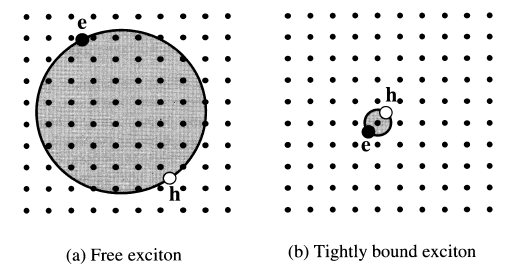
\includegraphics[width = 0.6\textwidth]{ch2/exciton}
\caption{Image that shows the characteristic difference between two types of excitons. Wannier-Mott excitons are not constrained to any atom and can move freely through the material in contrast to the Frenkel excitons which are much less mobile\cite{fox}}
\end{figure}

Stability of the exciton is strictly induced with the possibility of their potential to be big enough not to allow collisions with phonons.

\subsection{Photoluminescence}

Photoluminescence may be described as an emitted electromagnetic radiation as a result of its former excitation. The excited state depends on the internal energy structure of a radiated object and is an unique example of non equilibrium state. We might say from now on that during the whole luminescence process three possible scenarios are here to be observed. 
\begin{itemize}
\item Firstly the electron-hole pair is created.
\item The recombination process occurs.
\item Then the radiation escapes from our sample.
\end{itemize}

\begin{figure}[H]
\centering
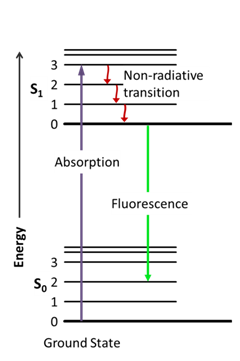
\includegraphics[height = 0.2\paperheight]{ch2/fluorescencediagram}
\caption{Example of few of the processes that are present during photoluminescence\cite{princeton}}
\end{figure}


The recombination is most probable near the surface of the sample, therefore the depletion of the carries is possible starting with the recombination processes with can be both radiative or non-radiative. Following that the recombination radiation is most usually emitted near the surface again, the great amount of experiments are created in the manner to directly look into the irradiated side.

The thing that luminescence can be accompanied to the absorption doesn't change the fact that it is quite different than it. In luminescence atoms emit light via the spontaneous emission so it's indivisibly defined by all of the vast majority of relaxation processes. The luminescence is divided into photoluminescence and electroluminescence. We can use it to study the bang gaps, transitions from it or transitions from deep doping states and defects. From the PL we can extract such informations as types and concentration of doping. Then, as we change the sample temperature we can also see how many relaxing centres are realised inside the medium. The possible relaxation types for exciton are shown in [Figure \ref{fig:relax}]
\begin{figure}[H]
\centering
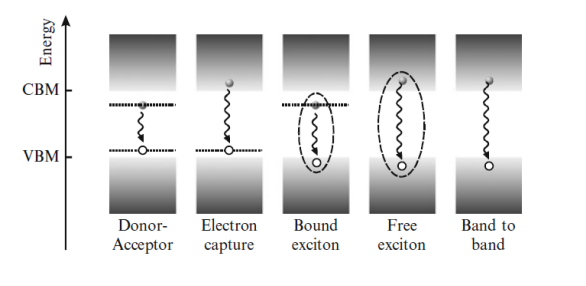
\includegraphics[width=0.5\textwidth]{ch2/recom}
\caption{Relaxation processes for excitons in the medium\cite{popko}}
\label{fig:relax}
\end{figure}

To describe spontaneous emission we can use Einstein A coefficient which is directly connected with B coefficient responsible for absorption and is different for different materials. When we have upper level populated at N at a time t we can say that:
\begin{equation}
\left( \frac{dN}{dt} \right) = -AN
\end{equation}
This tells us that emission behaves exponentially with $\tau_R $ being the radiative lifetime of a transition. The relaxation not always goes with photon emission, there can be a non-radiative one as well(f.e. as heat by creating lattice vibrations called phonons) and this is restricted by comparing the time-scales of emissions.  

\subsection{Quantum Confinement}

The properties of small systems are obviously rather different than those of bulk. The confinement in those kind of structures plays a crucial role in describing the physical properties. The first idea to describe semiconductors using quantum confinement and quantum mechanics methods has been used by Esaki and Tsu in 1970 \cite{Esaki1970}, which has lead to extreme advancement in describing the phenomena semiconductor physics. All thinks that are connected to optical properties of confined structures all directly derived from all the things that are connected to optical properties of solids described above. 

Changing the size of the crystal leads to great difference in the optical properties. The confinement effect in tiny regime leads us to the \textbf{Heisenberg uncertainty principle}, which tells us that the more we know the position of an object $\Delta x$, the less we know its momentum $\Delta p_x$

\begin{equation}
\Delta x \Delta p_x \geq \frac{\hbar}{4}
\end{equation}

This confinement leads to additional term to kinetic energy of particle with mass m connected to the uncertainty of momentum:

\begin{equation}
E_{con} = \frac{(\Delta p_x)^2}{2m}
\end{equation}

This energy can play an important part in its energy when it's comparable or greater than the thermal kinetic energy, which, let's say, on average is $\frac{1}{2}k_BT$.
This tells us that quantum effect will be considerable if the determined position is the size of $\sqrt{\frac{\hbar ^2}{mk_bT}}$. This can be transformed and stated that the position must be in the order of the \textbf{de Broglie} wavelength of an object $\lambda_{dB} \equiv \frac{p_x}{h}$.

Quantum confined structures are classified by the dimensions they are confined in.

\begin{itemize}
\item Quantum wells(confinement in 1-D)
\item Quantum wires(confinement in 2-D)
\item \textbf{Quantum dots}(confinement in 3-D)
\end{itemize}

The confinement of carriers in quantum dots describes that the carriers are completely localised on the particle. To describe the three dimensional confinement the model of the particle in a box has been used as a first method to the problem. Later on, it has been extended with more terms in the Hamiltonian like Coulomb interaction or non-parabolic and more complicated band structures. Those models have given rise to new properties such as: selection rules, radial wavefunction shape and the energy structures. This has shown that to truly understand the phenomena, we need to use non-linear optics as well. The beginning consists of going through one electron-hole pair(1EHP) states and then increasing the population and density of excited states by f.e differing the size of the nanoparticle. We will now state the 1EHP theory and tell where can it can be further explained. 

\begin{figure}
\centering
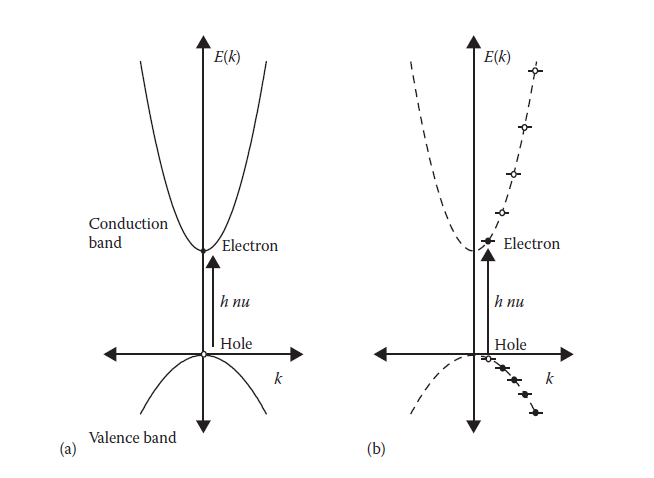
\includegraphics[width=0.65\textwidth]{ch2/energies}
\caption{The image of a band structure for two band model in direct band semiconductors a). In b) we can see that there are much more discrete states in a nanoparticle than in bulk a) \cite{Klimov}}
\end{figure}


\subsubsection{The Particle in a box}

This model is used in describing a behaviour of a particle with mass \textit{m} in a spherical potential with radius \textit{a}. \cite{Klimov} 

\[ V(r) = 
 \begin{cases}
 0  & r < a \\
 \infty & r \geq a
 \end{cases}
\]

where the radius can differ for holes and electron. This type of potential is connected with solving the stationary Schroedinger equation:

\begin{equation}
\hat{H}\Psi (\mathbf{r}) =  E\Psi (\mathbf{r})
\end{equation}

The potential containing the semiconductor sphere is relatively infinitely high. In that kind of environment, the wavefunction is a product of a Bloch function and a new envelope function. The periodic Bloch part shall be the same in the barrier and the well. 

\begin{equation}
u_k(r)_{barrier} = u_k(r)_well = u_k(r)
\end{equation}

The whole function now:

\begin{equation}
\Psi (r) = \psi (r) u_k(r)
\end{equation}

where $\psi(r)$ is the new envelope function for electrons and holes. We now have that(neglecting the other interactions - in single parabolic band approximation):

\begin{equation}
\hat{H} = \left[ \frac{-\hbar ^2}{2m_e}\nabla _e^2 \frac{-\hbar ^2}{2m_h}\nabla _h^2 \right] + V_e(\mathbf{r}) + V_h(\mathbf{r}) =
\end{equation}

The envelope function is separable for holes and electrons so the solutions have a shape like:

\begin{equation}
\Phi _{nlm} ^i(r) = Y_{lm} \sqrt{\frac{2}{R^3}} \frac{J_l(\chi _{nl}\frac{r}{R}}{J_{l+1}(\chi _{nl})}
\end{equation}

where $-l \leq m \leq l; l = 0,1,2,3...; n = 1,2,3,...$, $Y_{lm}$ are spherical harmonics and $J_l$ are the Bessel functions and $\chi _{nl}$ is the n-th zero of order l Bessel function. When we put effective masses we can estimate roots and calculate the energy levels for the envelope functions. Then we can calculate the optical properties calculating the overlap of the functions. Nevertheless, this approximation cannot fully explain what happens with the nanoparticles, we have simply neglected all the things that are making them different like Bloch functions, interactions etc. The next step would be to add interactions, mixing, splitting and then process to the other states as has been said at the beginning. This is rather Complex method, and the first thing you can do is to use the so called $k\cdot p$ perturbation theory to approximate some of the things and make calculations easier. As it is not the topic of the thesis, the places where you can read it further are here \cite{Klimov} \cite{ulrike} \cite{fox} \cite{dotsy}
\section{Theory of photovoltaic devices}
In this section we will provide the methods of solar cell characterisation and the quantities which are connected to it. More information can be rad at \ref{pv}

\subsection{Properties of sunlight}

The most important characteristics of the solar light are described by radiometric quantities. We will just state few of them. To finely describe the effects of sunlight we need to know:

\begin{itemize}
\item Spectrum of the incident light
\item Radiation angle
\item Radiant power density
\end{itemize}

\subsubsection{Photon flux}
$\Phi$ is simply stated as the number of photons per unit area in a fraction of time. We can then define the photon flux density to further divide it on the incident light wavelength. When we multiply $\phi _{\lambda } $ by the photon energy we get the energy per unit time, which is simply the power density. 

\begin{equation}
\frac{\partial ^2 P_\lambda }{\partial ^2 x^2} = \phi _ {\lambda } \frac{hc}{\lambda }
\end{equation}

\subsubsection{Spectral Irradiance}

It is most common quantity to describe a light source. It is the power density for a certain photon frequency. 

\begin{equation}
I_{e,\lambda } = \frac{\partial ^2 P_\lambda }{\partial ^2 x^2} = \phi_\lambda \cdot \frac{hc}{\lambda }
\end{equation}

\subsubsection{Blackbody radiation}

Derived by Planck, this radiation law is described with spectral irradiance\cite{planck}:

\begin{equation}
I_\lambda = \frac{2\pi hc^2}{\lambda^5(e^{\frac{hc}{k\lambda T}}-1)}
\end{equation}

\subsection{Solar Cell Operation}

For a solar cell to generate current, the following main processes must be present. First one is the possibility to absorb photons from incident light so we can generate carriers. We must remember that minority carriers are only stable for a minority carrier lifetime before recombination. Therefore, before this time, we need to collect those carriers to spatially disallow carriers to recombine. Ideally, if we create pair in the n region, the electric field sweeps the minority carrier through the junction to the place where it becomes majority carrier. In a short circuit situation, two carriers ideally meet together after flowing through the external circuit. 

The fact that the carriers must "live" through the distance needed to separate them is described by collection probability, which depends on the diffusion length and surface properties. 

The number of carriers collected in the solar cell compared to the number of incident photons describes the more macroscopic ability of the device. It is called a \textbf{quantum efficiency} $Q.E=\frac{number of carriers collected}{number of incident photons}$. It is strictly dependent also on the absorption so directly on the wavelength of incident photons. 

\begin{figure}
\centering
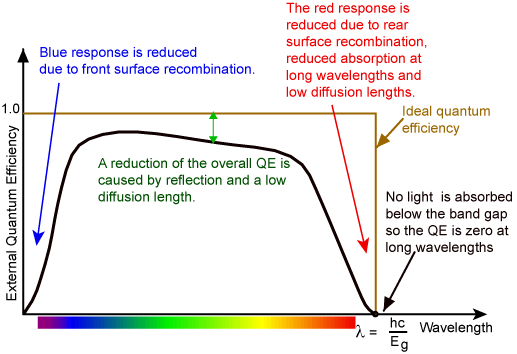
\includegraphics[width =0.6\textwidth]{ch2/QE}
\caption{Quantum efficiency of an ideal silicon solar cell \cite{pv}}
\end{figure}

It is also possible to describe an external QE, which also includes some optical effect such as reflection. 

\subsection{Solar Cell Parameters}
Here, we will state the most important parameters for solar cell characterisation, we will simply tell what do they stand for and how to measure them. 

\subsubsection{Short-Circuit Current}
$I_{sc}$ is the current that flows through the device providing that the voltage is zero across it(especially when we have short circuit). It comes directly from the generated carriers due to photogeneration and is connected to how well the structure can collect them or how strong the recombination processes are. It depends on:

\begin{itemize}
\item incident photons number(linear dependence on the incident power)
\item solar cell area
\item light spectrum
\item optical losses(f.e. absorption, reflection etc.)
\item real collection efficiency(its' probability)
\end{itemize}

We can clearly see, that this parameter allows us to differentiate between solar cells when comparing the ability to store generated carriers.(Remember, short-circuit current is not always the light generated current due to possible high series resistance).

\subsubsection{Open-Circuit Voltage}

$V_{oc}$ is the voltage that is maximally available when using the solar cell. For that voltage, the current through the circuit needs to be zero. It states the forward bias that we need to put to compensate the light generated current. $V_{oc}$ is logarithmically dependent on the incident photon power and it decreases linearly with temperature. 

\subsubsection{Fill Factor}

When speaking about the above short-circuit current and open circuit voltage we are meaning the maximal current and voltage that we can achieve in the solar cell. Of course, as the momentary power is just their multiplication, therefore, at those times when we get each of the two listed quantities, the power is equal to zero. In order to still describe maximal power of the solar cell, people tend to use the \textbf{fill factor} FF.

\begin{equation}
FF = \frac{P_{max}}{V_{oc}I_{sc}}
\end{equation}

where $P_{max}$ is the maximal power achieved by the solar cell. It is the   embodiment of the "squareness" of a solar cell. The higher the open circuit voltage, the bigger the FF. 

\subsubsection{PCE}

From the FF we can derive another, probably most useful quantity, which has been yet used in the former chapters. This quantity is the \textbf{power conversion efficiency} PCE. It is a ratio of energy from the solar cell to the summary energy income from the Sun. 

\begin{equation}
\eta = \frac{V_{oc}I_{sc}FF}{P_{in}}
\end{equation}

where $\eta$ is the PCE and $P_in$ is the sunlight power. 

\subsection{Shockley-Queisser limit}

Also known as a detailed balance. It was a derivation of an idealistic maximum efficiency of a solar cell based on a p-n junction made by Shockley and Queisser in 1961\cite{limit}. The most common form of the implementation comes with fundamental assumptions:

\begin{itemize}
\item We have finite mobility, so the collection of the carriers can be performed anywhere.
\item For wavelengths exceeding the band gap we have a complete absorption of photons.
\end{itemize}


In the principle, only photons with energy greater than the band gap can be absorbed and used in the generation of electron hole pairs. Generally, the electrons occupy the lowest level of the conduction band and so the exceed energy is released in heat in thermalisation process. For the idealistic model, they assumed that each photon with sufficient energy generates electronic charge q at voltage $V_g=hv_g/e$. $E_g$ is the threshold for energy as the band gap, and as we stated before, we assume that all photons are absorbed above, so the function a(E) is equal to zero below $E_g$ and unity otherwise. We can say that from the generated charge, the photocurrent density when shined with the photon flux $\Phi _{sun}$ is:

\begin{equation}
J_{sc} = q \int_0 ^{\infty } \Phi _{sun}(E)a(E)dE=q \int_{E_g} ^{\infty } \Phi _{sun}(E)dE
\end{equation}

Of course, to conceive the thermodynamic equilibrium, there needs to be an opposite process to absorption. We assume that the light emitted from the Sun is in the form of Blackbody radiation, as is the solar cell. The amount of radiation absorbed is the same as the emitted from the device to the environment with the same temperature. Therefore further it involves using a Planck Blackbody generalized formula for different energies above the band gap. Non-equilibrium radiation is only in a situation where the non-zero chemical potential of a radiation is present, and that is basically equal to a Quasi-Fermi level splitting(we have stated before that the splitting of a Fermi level is a non-equilibrium process). The photon flux emitted by a Blackbody with a bias voltage V is equal:

\begin{equation}
\phi (V,E) = \frac{2\pi E^2}{h^3c^2}\frac{a(E)}{e^{(( E-qV)/kT) - 1}}
\end{equation}

with c as the light vacuum velocity, k as a Boltzman constant, T as a temperature. This emission is connected with a recombination current density $J_r = q\Phi _e$, where $\Phi  _e$ is an integration of the flux density over all energies. In thermal equilibrium both currents are equal. When we apply voltage, we know that the current is a Shockley equation (Eq. \ref{eq:Shockley}. Maximal voltage is ideally the $V_{oc} = kT/qln(J_{sc}/J_{0} + 1)$, yes, it is the open-circuit voltage and $J_0 = q \int a(E)\phi _{abs}(E) dE$. Now, connecting this with AM1.5G spectrum Fig.(\ref{fig:AM15}), which is a standard spectrum for using solar cells, we can get that normally, for solar cells with band gap within 1eV to 1.5eV, we can get the maximal efficiency of 33\%  . \cite{limit}

\begin{figure}
\centering
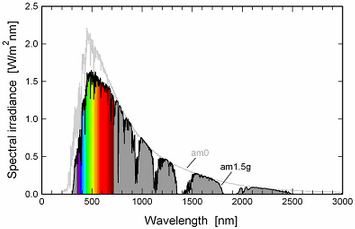
\includegraphics[width = 0.85\textwidth]{ch2/am15}
\caption{AM1.5 irradiation at Earth surface\ref{am} and AM0 at Earth's orbit}
\label{AM15}
\end{figure}

In exceeding the SQ limit we can use for example:
\begin{itemize}
\item Tandems
\item Magneto-optic devices
\item Hot carriers(strong electric field effects)
\item Multiple exciton generation(as in Quantum Dot Solar Cells it is possible to create more than one exciton from one photon!)
\end{itemize}

\subsection{Effective resistance}

To include some of the resistive effect on the solar cell and still use a model similar to the idealistic one, one uses series resistance and shunt resistance. Their main impact is on the FF of the device. Their dependence is on the geometrical properties of the solar cell. 

The series resistance has it's origin at three physical places: the emitter-base current, contact metal-semiconductor and top/rare contacts resistances. To include it we simply write the current equation as. 

\begin{equation}
I=I_{lg} - I_0e^{\frac{q(V+IR_s)}{nkT}}
\end{equation}

where n is an ideality factor and $R_s$ is the series resistance. The rest is taken from Eq.(\ref{eq:Shockley}).

For the shunt resistance the case is about the defects from the manufacturing. It simply takes away the factor $\frac{V+IR_s}{R_{sh}}$, where $R_{sh}$ is the shunt resistance. \cite{pv}
\section{Solar cell parameters}
\input{chapters/ch2/5}
\section{Quantum Dots and QDSCs - review}
\subsection{SEMICONDUCTING QUANTUM DOTS}

Due to their practical application and rather easy, yet not really repeatable fabrication, semiconductor quantum dots have made a vast impact in all technology. Their potential confinement in all three directions allows to profit from many new possibilities, not known in solid state physics before.
We can easily distinguish three different categories for their production which are:
\begin{itemize}
\item Self assembled QDs
\item Colloidal QDs
\item Electrostatically definded QDs 
\end{itemize}
Considering the fact that we are only using the second ones, we will mainly focus on them. 

\subsubsection{COLLOIDAL QUANTUM DOTS}
To put it straightforward, CQDs are semiconductor crystal of nanometre scale size, with diameter less than twice the Bohr radius, which are synthesized(deployed) by nucleation in colloidal solutions. They are surrounded and restricted by surfactant molecules called ligands. 

\begin{figure}[H]
\centering
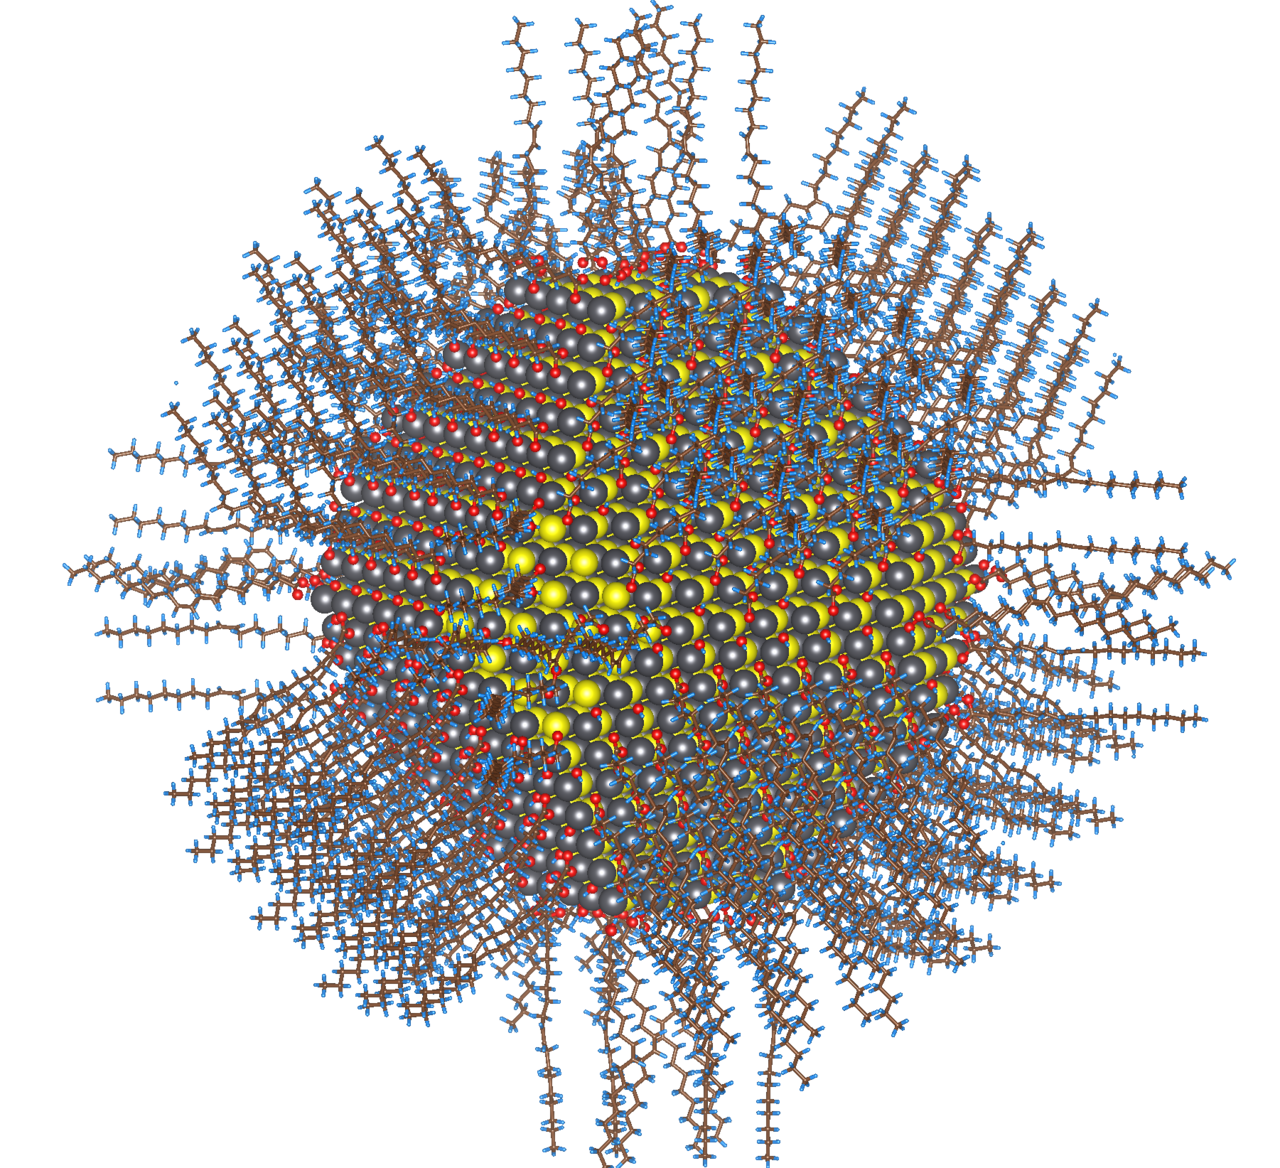
\includegraphics[width=0.4\textwidth]{ch2/colQD}

\caption{Image of ideal CQD composed of selenide with passivation with oleic acid, oleyl amine and hydroxyl ligands \cite{qd}}
\end{figure}

\noindent They have manifested to provide a development of numerous types of optoelectronic devices including photo-diodes and PV devices. The properties of CQDs are easily adjusted by changing the volumetric features of nanoparticles similarly to metallic nanoparticles in plasmonic transport. \cite{Abdelhady2015} \cite{G.D.Scholes2003}

\noindent Even though we don't focus on the synthesis of particular used CQDs, it is instructional and scientifically appropriate to be slightly familiar with it. It consists of three-component solutions, which are precursors, organic surfactants and solvents. In order for get the precursors transformed into single chains called monomers, the probe is heated to high temperature(they have enough energy to get separated), then, when there's enough of them, the monomers are growing into crystals. Of course, the temperature shall be manipulated with a dose of care because when it's too high the crystals aren't forming fine or at all. When we achieve optimal saturation of monomers, we get quite even growth of all particles, (small ones grow faster than the heavy ones) and it has to be sustained in order for the homogeneity to be achieved.
Typically, CQDs create alloys, binary or ternary, and contain 100 to $10^5$ atoms. Usually, they confine all carriers inside the volume.
\subsubsection{Quantum dot size}
With changing the size of the nanoparticle we can control the band gap over significant range of spectrum. Yet, practically, the width of the nanoparticle is estimated from the energy band gap.
 \cite{Yu2003}
 
\subsubsection{Quantum dot shape}
The geometry in physics plays an important role, there is no question about that. It is obviously not different for Quantum Dots. The quantum confinement strongly depends on the shape and dimensional geometry. The ability to control the growth of certain form allows the nanoparticles to exhibit a variety of properties. 

\subsection{CORE-SHELL CQDS}     
Modification of the standard synthesis methods allows us to create new behaviour and improvements in nano-structures characteristics. For example, in this method, same type, but different semiconducting nano-crystals are grown around the first ones(core). They tend to achieve better luminescence than the former because we simply drastically cut the possibility of non-radiative recombinations between energy levels. We can differ type 1 structures using conduction band of the core below the shell energy level(the core confines all carriers inside because of the energy minimisation) and in the second type, the energy levels are mixed so only one type of carriers is confined to the shell and the core. \cite{phdsemi}

\begin{figure}[ht]
\centering
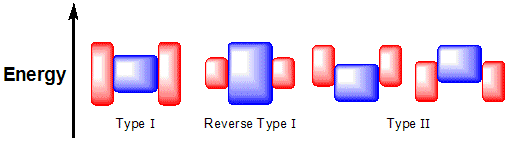
\includegraphics[width=0.8\textwidth]{ch2/Core_shell_types}
\caption{Types of Core-Shell CQDs(blue color is core energy structure), we can see that in the first type both electrons(smallest energy in CB) and holes(biggest energy in VB) are confined beneath the core. \cite{coreshell}}
\end{figure}

\subsection{CQD SUPER-CRYSTAL}
With CQDs we can even create super-lattices(layers of few materials which create a periodic structure). In order to achieve the fine quality of them we need to have an absolutely outstanding transport properties. \cite{tranSupLat}
\subsubsection{Further reading for CQDs}
More about synthesis and theory of nano-crystals and thermodynamics can be read in \cite{Klimov}, \cite{crystal}

\subsection{PRINCIPLES OF QDSCS}
Quite early, because in fair 1960s, the idea of harvesting sunlight with using sensitized semiconductor devices with generation of carriers inside narrow band semiconductors has been proposed. The usage of colloidal quantum dots has produced new possibilities and and shown amusing prospects for using nanotechnology. The properties can be tuned by changing the QDs size itself which means changing the size of electronic band (relocate CB - conduction band and VB - valence band) depending mainly on effective masses of the carriers. The electronic shift that we can achieve by relatively simple parameters manipulation will provide a shift of VB edge downwards and CB upwards, as a result of a, quite important in this scale, quantization of energies. As we know, besides band gap enlarging, it also changes the driving force for carries injection and this is most important part, as we want to use them as an amplifier in the PV devices. The great achievement of these types of solar cells is the decoupling the charge generation and its transport to different materials- the hole and electron transport layers. The effect of such a procedure is the decrease in recombination process and reduction of production costs.  Without that technique, the architecture is adequate to the standard PV solar cell device. The generation of electron-hole pairs proceeds the injection of electrons from CB of light harvesting material to electron acceptor layer and holes from VB to hole acceptor layer. We call this process a charge separation. Nevertheless, even though we do regenerate QDs in the light harvesting area after charge separation, we still have to struggle with recombination processes and consider them as the significant performance wasters. \cite{S.Gimenez2009}


There are few commonly used configurations of solar cells based on those previously mentioned nano-crystals and are shown in \ref{fig:confstru}

\begin{figure}[ht]
\centering
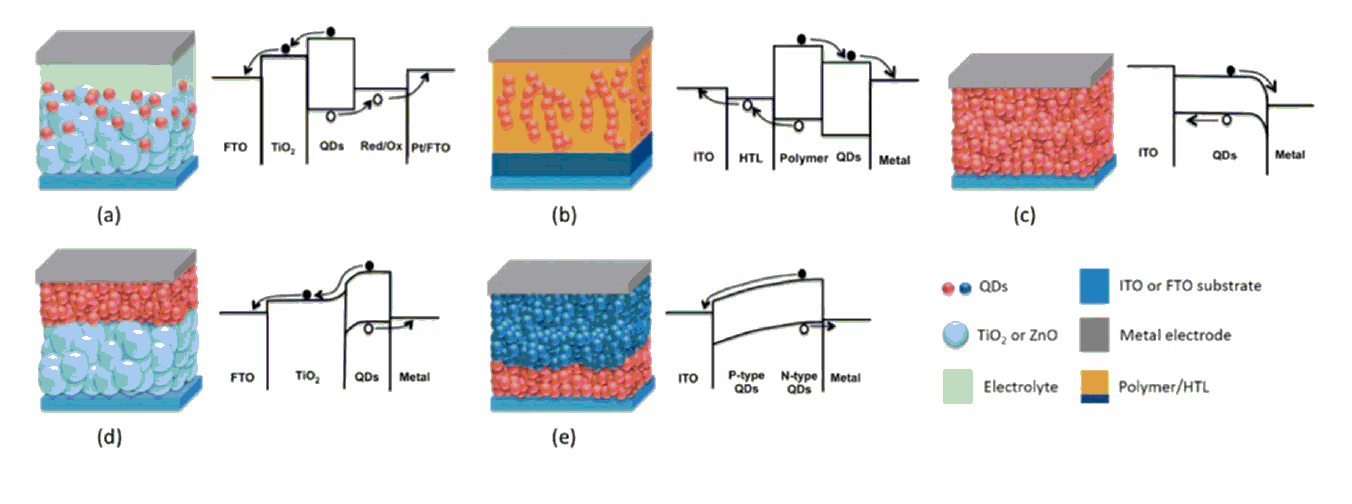
\includegraphics[width=\textwidth]{ch2/confstru}
\caption{Schematic illustration of configurations and band structures of QD solar cells: a) QD-sensitized b) hybrid QD-polymer c) Schottky junction d) p-n hetero-junction e) p-n homo-junction \cite{HuashangRao2018}}
\label{fig:confstru}
\end{figure}

Schottky schematic is a type of device where thin QDs film is placed between two contacts and is used for generating electrons and holes. The barrier, which is created between the low-work metal and QDs layer, is quite similar to bulk one where the potential is bent proportionally because of the charge transfer between the layers that touch. From them, few very unique and promising short currents have been achieved. Unfortunately, low open circuit voltages are present for them because of the pinning of Fermi level. Then, we have the depleted heterojunction, where we use wide band gap oxides such as ZnO on a conducting glass. After that we put some QDs films above that and end it with a fine metal contact. The oxide layer behaves as layer for electron conducting phase, so the metal contact extracts majority carriers. There we have more of a compromise between $I_{sc}$ and $V_{oc}$.  The next type is a hybrid QD-polymer solar cell, where electron is transported and photon absorbed both in the QDs layer(with the polymer film together). The PCEs of such attitudes to the device engineering is still smaller than the former ones, probably due to not optimal hole transporting layers. P-n hetero- or homo- junctions are both traditional methods of harvesting and transporting the light but instead of using bulk semiconductors, we use semiconducting QDs. 

The Quantum Dots Sensitized Solar Cells(QDSCs) are devices in which QDs are not the most important part when considering the carrier transport. The idea was to replace dyes with QDs, but the rest of components has been still based on the concepts formed by their ancestor. Sadly, not to late after, it was realised that it's not so similar at all and some of the components need to be redesigned from scratch. However, even though the DSCs are easier to achieve the better performance with, the QDSCs are more promising and theoretically can be cheaper and have longer lifetime. Inside the device structure, the QDs itself are responsible for light absorbing and carriers creation. Then they are divided in different layers so obviously the great PCE can only be achieved if large incident photon to current efficiencies(IPCE), $V_{oc}$ and fill factor are possible. 

\begin{equation}
IPCE(\lambda ) = LHE(\lambda ) \phi_{inj} \eta_{col}
\end{equation}

Where $\eta_{col}$ is electron collection efficiency, $\phi_{inj}$ is electron injection efficiency and of course $LHE(\lambda )$ is left to be the light harvesting efficiency, so it's directly connected to absorption and automatically to QD loading and the band gap, as has been seen in theory chapter. The loading only depends on the quantitative parameters of transport oxide layers such as thickness, particle size and coverage degree. The injection then depends on how fine would we attach both layers together and the collection efficiency will consider the interfaces and the internal structure of transporting phases. Of course this means, as in all of the solar cells, high mobility with relatively slow recombinations in the main energy regime. We can now clearly see that the big advantage of those cells is that they separate the ideas of charge generation and transport to different parts, so it gives more possibilities to engineer new materials. 
\cite{HuashangRao2018} \cite{Wu2014}

\subsection{MATERIALS AND PERFORMANCE DEVELOPMENT OF QDSSC - A REVIEW}

\begin{enumerate}

\item \textbf{Electron Transporting Materials(ETM)}

They are used to support charge separation as briefly described above.The function proceeds as a support for QD in the charge generation layer, as it transports charged electrons to the conductive substrate(usually ITO or FTO). \cite{X.Gao2017} \cite{Tian2015} The properties shall be as follows:
\begin{itemize}
\item
  Matching CB edge which will determine exciton generation and
  partial transfer efficiency.
\item
  High electron mobility.
\item
  Fine surface to provide suitable loading of particles.
\item
  Suitable technological properties, such as stability, low cost etc.
\end{itemize}

The most widely studied materials nowadays are TiO2 and ZnO. Materials based on the first one are of such importance due to their non-toxicity, chemical stability and low cost \cite{I.Mora-Sero2014a} \cite{Tian2015} . Among them (TiO2-NP) based mesoporous layers are researched as photo-anodes \cite{I.Mora-Sero2014a}. The highest efficiency ever recorded(up to 2018) were based on that material \cite{Du2016} \cite{J.Du2017} . Unfortunately, the probability for charge recombination in that kind of films is rather unsatisfactory.  Therefore, one provides one-dimensional structures such as nano-rods and nano-wires to maintain fairly smoother electron transport channel and decrease loses provided with recombination \cite{Y.Liu2014} \cite{M.A.Manthrammel2015} . In 2007 it was shown that TiO2 nano-tubes win over nano-particles of the same material in case of transport capacity \cite{Kamat2009} \cite{Tvrdy2008}.  Thus, the research of such structures was accelerated and many brand new CdSe sensitisation methods were proposed \cite{A.Yamada2010} . After that, many different sensitisations were provided, in which also PbS QDs had their small part \cite{C.Shi2017} . Although promising, the 1D structured TiO2 based anodes were unsatisfactory in case of PCEs, when comparing to standard nanoparticles (maximum of around 6\%  ). The hypothesis was put on insufficient loading amount on 1D structured TiO2, therefore the focus should be put on improvement of that area. A group of researchers has also used graphene frameworks incorporated into TiO2 photo-anode achieving 4.2\% PCE for QDSSCs. \cite{XinMeng2014} By using double-layered films with particles of bigger volume, there has been achieved a high PCE of 4.92\%. A lot of dopants and different solutions, hybrid photo-anode films with metal and non-metal ions and carbonaceous layers has been proposed to improve performance of PV devices. Also with the usage of hollow structure techniques, by creating nano-tube arrays, the possibility of achieving a PCE of 6 \% has been shown \cite{MikhailArtemyev2019}. Improvement in light absorbance was achieved by using microporous TiO2 photo-anode for PbS quantum dot sensitised solar cells achieving up to 3.5\% PCE performance.

In case of ZnO based photo-anodes the differencing property is a higher electron mobility and better conduction band edge. With them, the achievement of higher $V_{oc}$  is more probable \cite{X.Gao2017} . Unfortunately, the chemical stability of those films is significantly lower. Similarly to the former, the nanoparticles were widely studied. \cite{L.Lv2014a} As an example, the CdS sensitised ZnO nanoparticles were used to construct a photo-anode, which allowed the achievement of 4,46\% PCE. They used TiO2 passivation of ZnO surface to improve the PCE of same sensitized CdS/ZnO QDSCs by more than 2\%, achieving 4.68\% \cite{Zhang2013b}. Similarly, the 1D structures for ZnO can be crystallised. The distinction from the former is the ease of it's development. The ZnO nano-wires sensitised with CdSe constructed in 2007 were the launch of the technology development and allowed Young et al. achieve PCE of 4.15\% \cite{J.Qiu2013}. Many more one dimensional structures of ZnO based photo-anodes were used to research maximal performance but it was shown that the problem again concerns the surface area \cite{Gonzalez-Pedro2015}. The second strategy to improve the performance of such material based structures is double layer replacement with two different 1D structures such as NR on bottom and TP on top.  However, the PCEs of ZnO based films still stay behind TiO2 ones.\cite{Zhang2013b}  The Al/Cl hybrid doping allowed to use ZnO in IR spectrum.

There are other kinds of ETMs researched as well.  Using big tandem structures has manifested superb PCE through simulations \cite{GregoryF.Pach2017}. The doping of synergistic fullerene electron transport layer has proven to increase solar cell performance \cite{OleksandrVoznyy2014} . A series of materials such as SnO2, NiO, BiVO4, Zn2SnO4,BaTiO3, CoO have been incorporated to QDSC manifesting future potential. High performance has been achieved using CdS thin films as single-source precursors to ETM layer providing over 8\% PCE. \cite{RobertJ.Patterson2017}

All of the above materials are n-type semiconductors. Furthermore shall we proceed to introduce the p-type metal oxides and p-type Quantum dot sensitised cells. Typically, the NiO semiconductor is widely used. The promising and comprehensive material that can be implemented is CuSCN, which is an inorganic of p-type. Of course, the extraction of a hole from light harvesting layer to a redox couple will be rather slower than in case of electron. Therefore, being the potential solution to this problem, the p-type semiconductor based layers are beginning to leave their mark in PV devices. As expected, the most accurate application of that type of films would be the tandem configuration construction, which contains both n-type and p-type QDSCs to overcome so called  a Shockley-Queisser limit. However appealing, the efficiencies of p-type QDSSCs are yet to be enhanced.

\item \textbf{Hole transporting material (HTM) layers}

The electrolyte or HTM is crucial to QDSSCs as well. The properties of
such film shall be:

\begin{itemize}
\item
  Low corrosivity.
\item
  Red-ox potential appropriate to regenerate QDs and maintain fine
  V\textsubscript{oc} .
\item
  High conductivity through ions.
\item
  Stability and transparency in visible spectrum.
\item
  Possibility to fully regenerate. \cite{HuashangRao2018}
\end{itemize}

The common electrolytes:

\begin{itemize}
\item
  \textbf{Liquid electrolytes}
\item
  \textbf{Quasi-solid state electrolytes}
\item
  \textbf{All-solid state electrolytes}
\end{itemize}

were described comprehensively in the following research papers \cite{HuashangRao2018} \cite{Zhang2015} \cite{Song2017}

Although using Sb\textsubscript{2}Se\textsubscript{3} as a thin light
harvesting film, a group of researchers has also used PbS colloidal
quantum dots as a hole transport layer achieving 6.5\% PCE in 2017 \cite{Wang2017}. Earlier, the usage of graphdiyne(a novel large $\pi$ -conjugated carbon hole transporting material) has allowed an efficient hole transport layer for solar cells based on PbS-EDT colloidal quantum dots\cite{MingjianYuan2016}. Before that, in 2015, colloidal CuInS\textsubscript{2} QDs were layered to hole transporting solution and, even though the scientist did their research on Perovskite solar cell, they accomplished to get almost 8.5\% PCE\cite{JunZhu2015}. The extended device stability and a rise to 10.6\% of PCE was certified using CQD solar cells using P3HT as a hole transport material \cite{Zhang2016}.

\newpage
\item \textbf{QD sensitizers }

The main part of our PV device, the QDSC are QDs. The ability of harvesting interfering light is a crucial component of such device. \cite{Ikeda2014} Therefore, the ideal nano structures should exhibit certain properties:

\begin{itemize}
\item
  A higher conduction band edge than the one in the electron transport material and lower than in hole transport material to provide effective charge separation.
\item
  Obviously, as in all semiconductor PV devices, we shall provide a
  material with accurate band gap, ideal for our purpose. The reason is
  clear, we are interested in superb absorption in wide range of solar
  spectrum.
\item
  The stability is the crucial property as well.
\item
  From the technological point of view - the simple preparation and of
  course low toxicity would be rather expected.
\end{itemize}
Therefore, we will now examine methods to deposit them and the
differences between certain QDs materials.

\textbf{Deploying on the surface}

Because of QDs being inorganic and possessing larger size than simple
molecular dyes, they are much more difficult to tether onto metal oxide
to form a high quality mono layer. Therefore high QD-loading amount is
rather high to achieve. We can difference the deposition methods by
putting them into two categories: \emph{in situ} and \emph{ex situ} . In
the first one, the QDs are grown directly on the surface of the metal
oxide substrate, being created using an ionic precursor. We can include
chemical bath deposition(CBD) and successive ionic layer adsorption and
reaction(SILAR) into this category. The second approach bases on pre
synthesising of QDs and then depositing them onto the metal oxide.
Easily processable and finely reproducible, the in situ method has been
used more widely than its' counter. In that kind of deposition we can control not only the QD-loading amount but also size distribution.
Unfortunately, the achieved density of trap states is rather high, therefore the obtained maximal PCE is about 7\% \cite{L.Lv2014} . In this case, excluding the QDs growth process, we have to accurately deploy them onto the surface. The most common methods are: direct absorption, linker-molecule-assisted self-assembly, electrophoretic deposition. \cite{HuashangRao2018}

\textbf{Ligands}

The ligand part in QDs is, as mentioned before, the important part of obtaining high efficiency of QDSCs \cite{Shang2016}. The comparison of halide ligands in PbS CQDs for field effect transistors(FETs) has been made by researchers in 2018\cite{Balazs2018}. The capping-ligand-induced self-assembly method was the clue for TiO\textsubscript{2} photo-anodes\cite{HuashangRao2018}. Nevertheless, researchers haven't discovered a satisfying approach yet. In 2012, the deposition method were optimised through using ligand-exchange techniques.\cite{Cheng2012} Thanks to that, the PCE record of 13\% was achieved \cite{W.Feng2018} . Not only CLIS deposition has been used. The aqueous solution provided the simplification of QDs fabrication with shorter ligands. Some relatively high PCEs have been achieved with that method. Then, the organic  molecules usage allowed scientist in 2015 to achieve 3 times bigger PCE compared to common creation of PbS quantum dots.\cite{Infante2015} The certified PCE of 11.21\% has been achieved via so called ``solvent curving'', which is the simplified method of PbS QDs fabrication processing. The passivation of PbS QD surface with
L-glutathione was used to produce QDSSCs with promising results.\cite{Cordes2016} 10.6\% PCE was achieved thanks to solvent-polarity-engineered halide passivation \cite{OleksandrVoznyy2016} .


\textbf{Binary structures}

Up to date, binary QDs have also been used as sensitizers. There are
many examples but the most common are: InP, InAs, CdS, CdSe, CdTe,
Ag\textsubscript{2}S and with them, the most interesting one considered
in our case - PbS.\cite{P.Zhao2015} \cite{Y.Yu2008} The main problem with
them is to control and balance the narrower band gap and relatively high
conduction band edge. For example, for PbS nano crystals the band gap is
narrow, but the conduction band edge is rather low, which causes the
problem and has to be dealt with. In case of binary QDs we have to
balance between the light harvesting efficiency and efficiency of charge
injection. Mixing binary structures (for example PbS with PbSe) has been
also proven to enhance the interesting efficiency\cite{ShujuanHuangb22019} \cite{Fan}. Treatment of PbS QDs with metal salts provided some advantages in CQD PV devices resulting in the increase of short circuit current and fill-factor \cite{Maurano2016} .
The crucial part of success in getting high efficiency would also be
suitable engineering of solvent\cite{YuehuaYang2017}.

\textbf{Core shell QDs usage}

The other methods to use QDs as sensitizers in PV devices is creating a
Core/Shell QDs. Their unique properties have been mentioned before. The
alignment in these provides ability to tune the light-absorption range,
recombination processes and charge separation. Usage of them in QDSCs is
rather modern. The first noticed implementation was created by Lee et
al. in 2009. Through SILAR method, he achieved PCE of 4.22\% \cite{Lee2009}. Yet the difficulties in creating specific materials may occur, because of inability to prepare a stable precursor for deposition methods. 

\textbf{Alloyed QDs usage}

The massive perspective in PV devices has also been established by using Alloyed QDs. These allow us to create the non-linear band gap \cite{Regulacio2010} . Stability in such materials is again much higher than in their constituents. A lot of scientific research was done in that area.

\textbf{Doping}

We can also include dopants to QDs. There were a handful of propositions in the \cite{HuashangRao2018} review. Yet, the promising idea has been introduced with the usage of metallic nanoparticles dopants by considering plasmonic physical phenomena.\cite{Kubo2015} \cite{YongjieWang2017}

\newpage
\item \textbf{ Counter electrode}

As we may already expected, they are also playing an important role in
achieving high performance of PV device. The electrodes have to catalyse
reduction reaction. These shall poses properties as follows:

\begin{itemize}
\item
  Good conductivity
\item
  High catalytic activity
\item
  Fine stability, either chemical and physical
\end{itemize}

We can also put them into four categories:

\begin{itemize}
\item
  \textbf{Noble metals}
\item
  \textbf{Metal chalcogenides}
\item
  \textbf{Carbon materials}
\item
  \textbf{Composite CEs}
\end{itemize}
\end{enumerate}
Recent progress has been comprehensively described in those publications.
\cite{Yang2017} \cite{HuashangRao2018} .

\chapter{Preparation and deposition methods and experimental parameters}

\section{Quantum dots purification}
After the synthesis, the lasting of many redundant impurities inside the solution provides unwanted complications such as lower photo-luminescence, faster oxidation or potential problems with the traps. Therefore, separating our beloved nano-crystals would be crucial for achieving the purity of the device. The  impurities that did not react during the process are a large scale particles that can be  filtered by many different methods. \cite{Shen2017}\cite{purif} To do that, people usually change three main properties of the QDs solution which are: polarity, size and mobility. For any colloidal system, the challenge that we approach is not only connected with the type and the amount of ligands connected to the core crystal but the solvent properties as well so the parameters may change in a real time for any of the part and we need to be really careful not to change any drastically. 

\subsection{Purification method}

For our case of PbS nano-crystals, the method used was a polarity based purification technique. There are two most common processes in which we can clear the untidy system when considering only polarity. It is either precipitation and re-dissolution (PR) method or extraction method. 

The first one is frequently used in case of non-polar solvents and thanks to the anti-solvents introduction the polarity of the solution is increased. Then, the retaliation of the impurities via the supernatant(which is the mixture that is floating after the centrifugation of the suspension) is taken away and we are left with quite pure nano-crystals which can be the redissolved in clean solvents. The repetition of the process is available for us for several times but not infinitely, because we can misleadingly get rid of ligands, which are necessary in chemical non-static processes that occur inside the solvent. It has also been seen for many times, that larger particles are more able to participate in the polarity induced precipitation than the smaller ones which means it's harder to get rid of the later ones. The method isn't always accurate because of the ability of the ligands to dissolve which can be really similar to the nano-crystals. More can be read in publications mentioned in the beginning of the chapter.
\vline

\subsection{Method's properties}
\label{subsection:CHXpurification}

\subsubsection{CHX/Acetonitrirle polar purification.} 


The first thing to do was to add chloroform to the nano-particles dissolved in CHX solution. CHX is the standard cykloalkane used in case of quantum dot nano-crystals. The amount of the liquid was about the former amount of CQDs solution. Then, to begin it's work as a purification mixture, we added polar solvent acetonitrile. The unwanted particles and some of the wrenched ligands are then separated using the centrifuge. Carefully, in the nitrogen created vacuum, we separated the supernatant because of the danger of PbS fast oxidation. Chloroform was then again used as a solvent for now clean CQDs.



\section{Depositions parameters and methods}
After successfully purifying the Quantum dots, the time for the deposition has came. We will now discuss used methods and then show the schematic for the steps taken in creating the device. 

\subsection{Glass contact cleaning}

To be sure that we can reduce a number of defects connected with dust and air pollution, the transparent glass contact needs to be cleaned. It it done with simple method using a strong detergent and solvent(in our case isopropanol). The glass is placed inside the holder and put in deionised water for rinsing. After few times, when the glass is clean it is then placed in the UV-ozone cleaning chamber. Inside, UV lamp either dissociates Oxygen into triplet and then it combines with $O_2$ generating ozone or with the higher wavelength dissociates $O_3$ and makes singlet oxygen in the process(it reacts with substrate surfaces strongly). It is a dry process, in which there is a low damage on the probes. 

\begin{figure}[ht]
\begin{subfigure}{.5\textwidth}
  \centering
  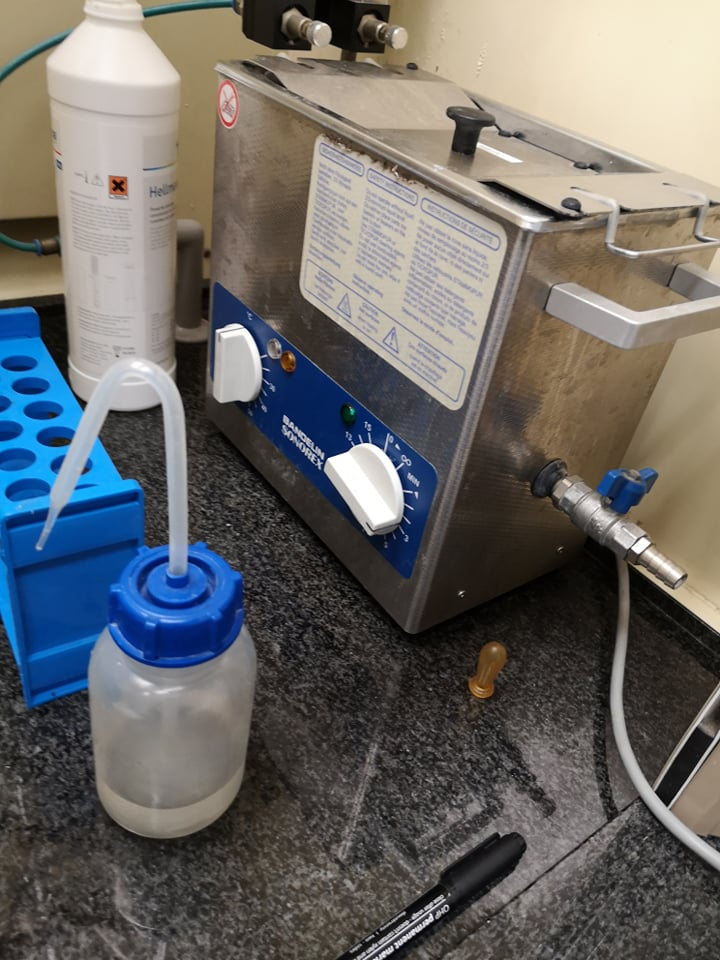
\includegraphics[width=.8\linewidth]{ch3/sono}  
  \caption{Ionized water cleaning equipment}
\end{subfigure}
\begin{subfigure}{.5\textwidth}
  \centering
  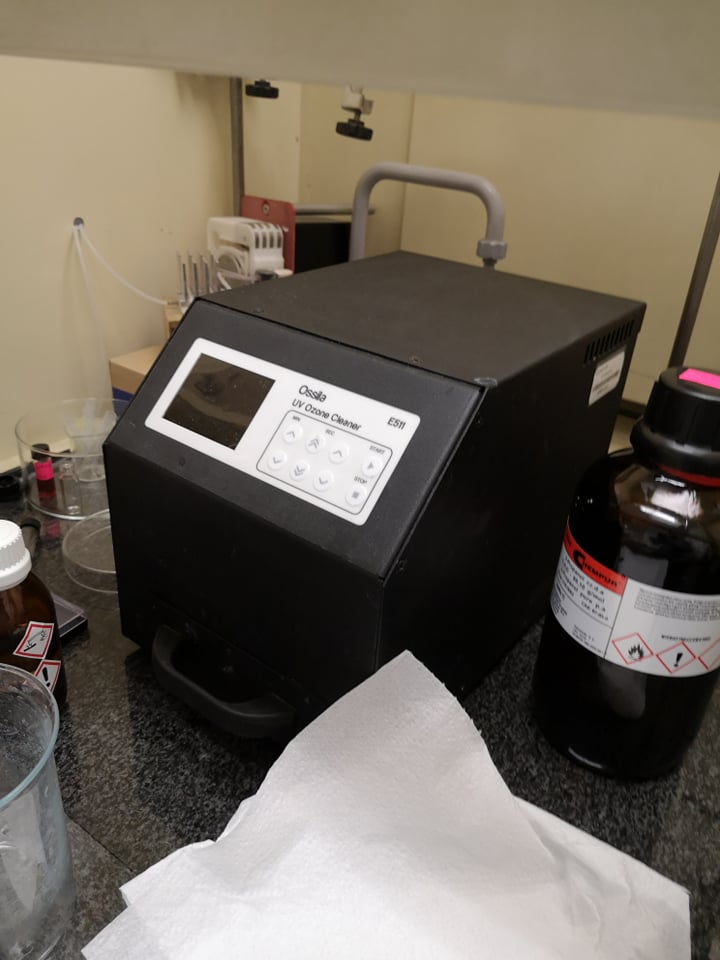
\includegraphics[width=.8\linewidth]{ch3/uv}  
  \caption{UV-ozone cleaning equipment}
\end{subfigure}
\caption{Cleaning methods environment}
\label{fig:clean}
\end{figure}

\subsection{Spin Coating}
To achieve an uniform deposition, the technique of applying a small amount of rotating material is used. The centrifugal force achieved with rotation allows to place the substrate only if it's possible to convey it on the surface for a longer period. Usually, as also in our case, the substrate can simultaneously evaporate during the process. With the angular speed, the thickness of a layer is parametrized, so higher the velocity, the thinner the layer. 


\begin{figure}[H]
\begin{subfigure}{.5\textwidth}
  \centering
  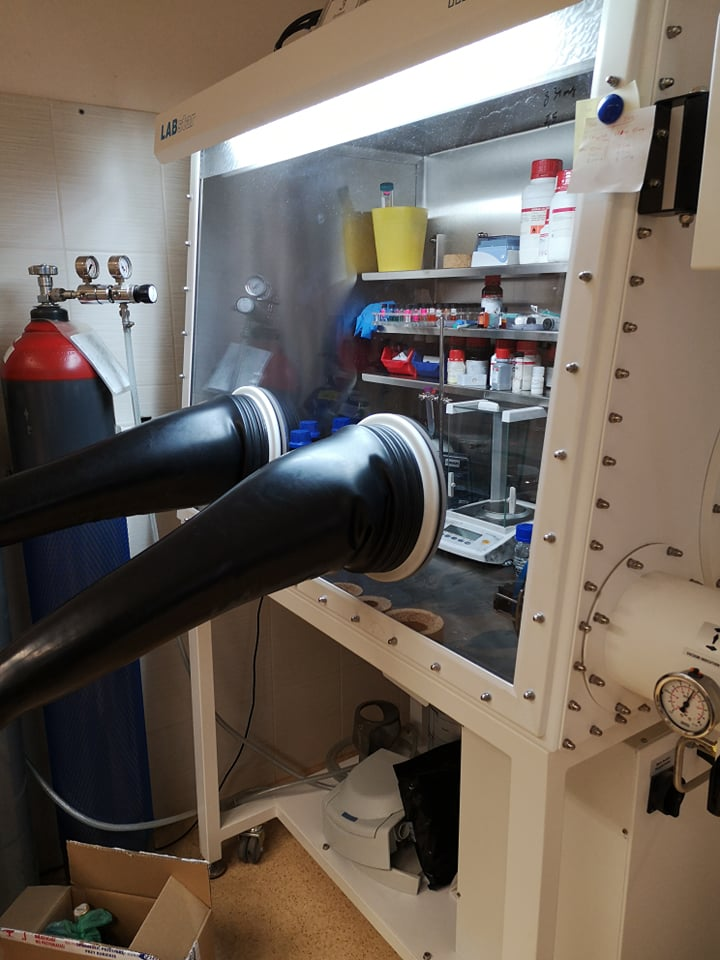
\includegraphics[width=.8\linewidth]{ch3/glovebox}  
  \caption{Glovebox used in the laboratory}
\end{subfigure}
\begin{subfigure}{.5\textwidth}
  \centering
  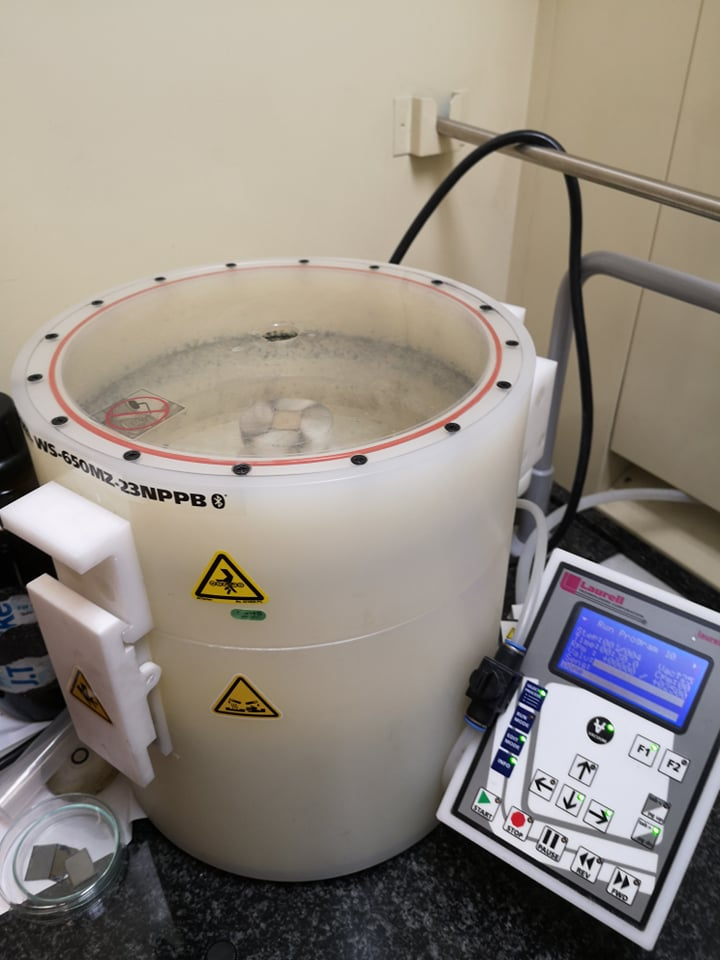
\includegraphics[width=.8\linewidth]{ch3/spincoater}  
  \caption{Spincoater used in the laboratory}
\end{subfigure}
\label{fig:gloves}
\caption{Laboratory equipment view}
\end{figure}

\subsection{Glovebox}

It has to be highlighted that some of the processes cannot be done with the contact of air. Therefore, a single machine called glovebox is used to overcome some of the task and to ensure even higher quality of the out-coming creation. Inside it, the inert atmosphere is made with using nitrogen so the items need to be inserted with vacuum pump.
\newpage
\subsection{Sputter deposition}

\begin{wrapfigure}{r}{0.401\textwidth}
\centering
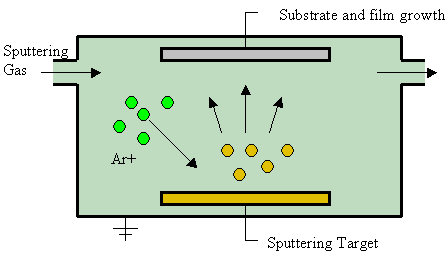
\includegraphics[width=0.4\textwidth]{ch3/sputter}
\caption{Sputtering deposition schematics(\url{https://www.wikiwand.com/en/Sputter_deposition})}
\end{wrapfigure}
After creating the distinct and separate layers for transporting and absorbing parameters we have to create a second contact for the device. 
In our case, the sputtering method PVD is used. It uses a material called a target(an item consisting of a desirable material) from which parts are ejected into the substrate. The sputter gas is pumped into the chamber, where a magnetic and electric fields are both confined. The gas atoms thump target ions which create the plasma in the chamber and then they hit the substrate. 

\begin{figure}[t]
  \centering
  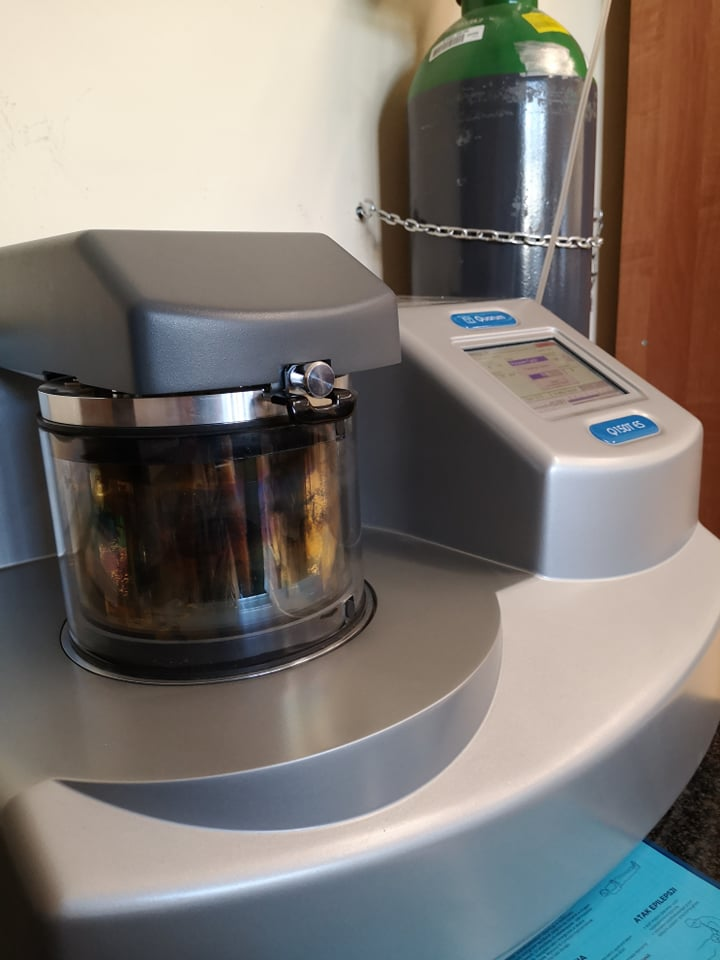
\includegraphics[width=.4\textwidth]{ch3/napylara}  
  \caption{Sputtering deposition device that we were using}
\end{figure}






\chapter{Results}

\section{PbS Quantum Dot Solar Cells}


The whole idea of all-solution processed QD solar cells is beginning to mark its footprint in modern photovoltaics. Within all of type III SC PbS QDs are promising candidates and certainly a field of quick improvement. Yet, what is so promising about them and what are the features that distinguish them from other types. 
In case of PbS QDs it must be denoted that the main advantages that they provide are the high efficiency and wide bandgap tunability due to its direct link with quantum dot size. For photovoltaic purposes the next important thing would be the ability to multiple excitation through the band gap. 
\begin{wrapfigure}{l}{0.601\textwidth}
\center
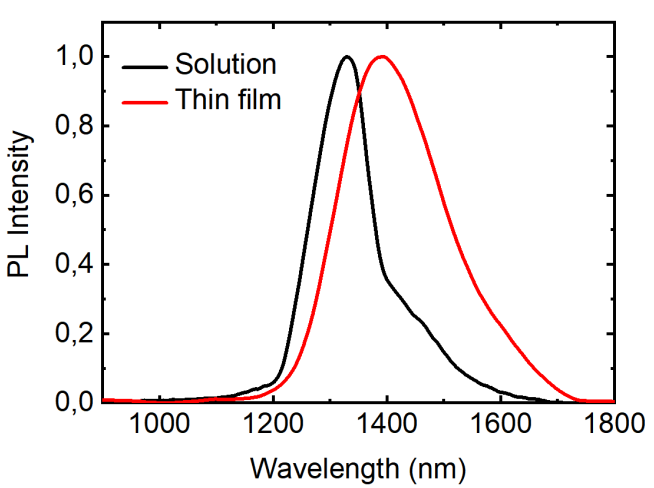
\includegraphics[width=0.6\textwidth]{ch5/Pbs-QDs1st_emm}
\caption{Emission spectrum of used PbS QDs \cite{2011}}
\end{wrapfigure}
They are used in many different structured solar cells, creating a numerous variations of junctions and quantum dot treatments and achieved over 11\% power PCE as for last few years. The main problems with them would be to conduct and choose a fine ligand passivation. In our case the halide anions from precursors of tetrabutylammonium iodide (TBAI) and 1,2-ethanedithiol (EDT) were used. Ligands from such precursors do not only, more or less precisely, passivate surface defects, which are of course bad for our case, but modify electronic properties of QDs as well. The PbS-EDT layer was used as hole transport and  PbS-TBAI, a main light harvesting layer,  has been reported to usually be a n-type semiconductor, probably owing to a) I¬  anions that are exchanged in PbS QDS with S¬2- and b) I- anions are bound to the surface and repulse a oxidative processes. The choice of those were due to rather improved stability of QDs comparing to other layer passivating (devices with TBAI and EDT bi-ligands have been shown to provide a much longer stability in air than others). Although a longer air-exposure provides undesirable consequences that downgrade the cell significantly, the short period exposure is suspected of creating a more efficient charge extraction. Nevertheless, the inner processes that allow that bi-layer structure to be one of the best, provided for those types of QDSCs, is still eluded and further improvements are expected if it becomes much more understood. For example, a greatly simplified deposition has been achieved by replacing methanol with acetonitrile, which consequently improved electrical properties of photovoltaic device as well. (The device structure was very similar to ours). There are irrefutable results in achieving fine results from synthetisation from the group.\cite{Wang2017} \cite{Hu2016}
\subsection{First device deposition}
\begin{figure}[t]
\center
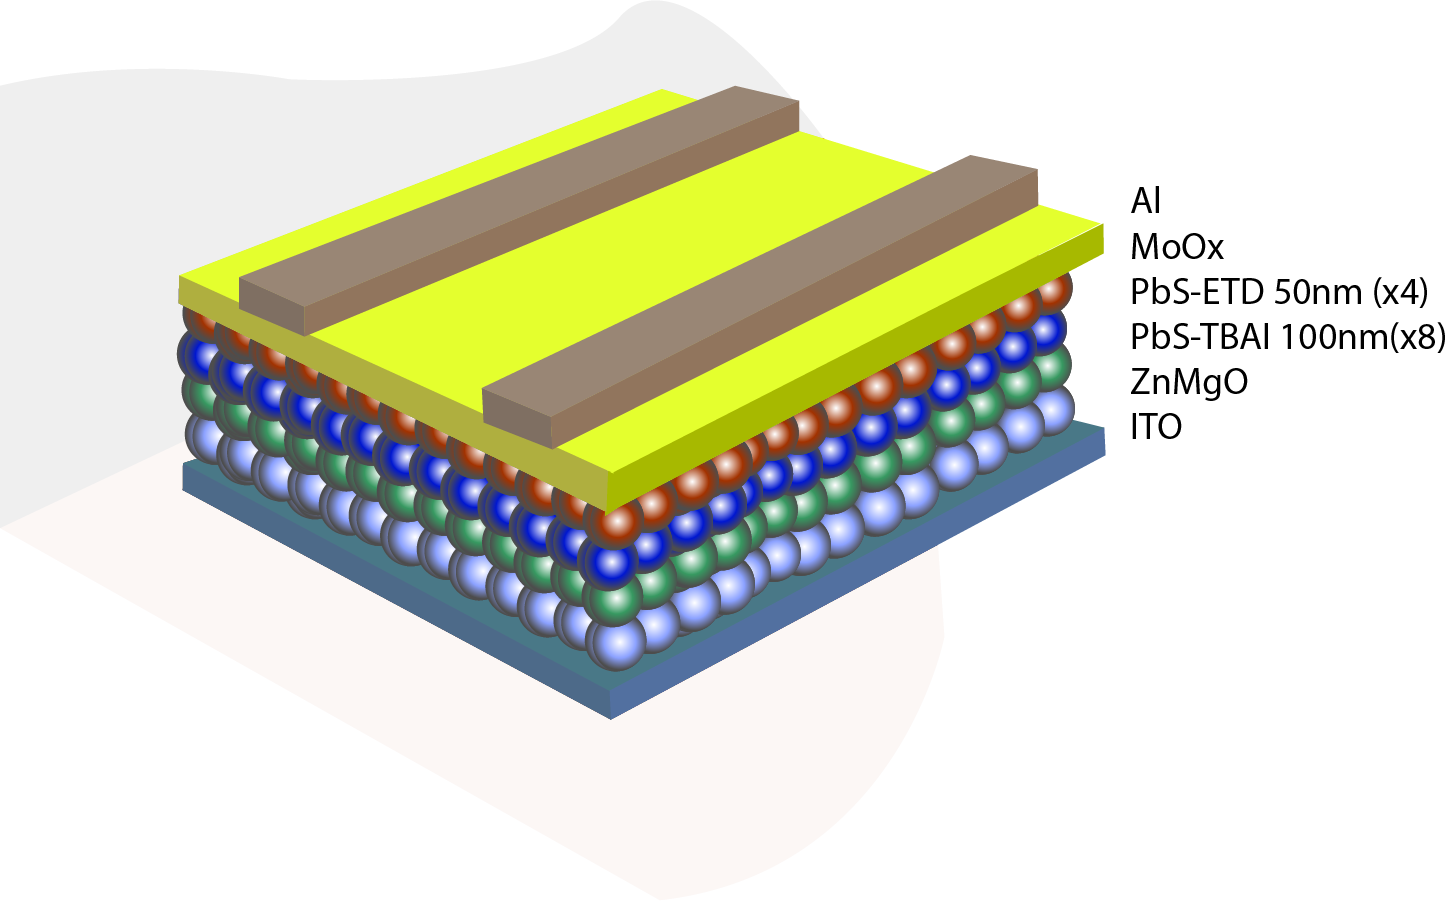
\includegraphics[width=0.7\textwidth]{ch5/3DStruct}
\caption{3D structure of the first device based on PbS QDs}
\label{fig:1stStructure}
\end{figure}
A first insight of what can we do and what would be the challenges to overcome has been made due to creation of a first working solar cell. The cell was based on PbS QDs and it has shown a promising quantities for further development. The whole subchapter provides a comparison of Vimun $3^{rd}$ generation silicon solar cell and our own QDSC.
\begin{figure}[H]
\center
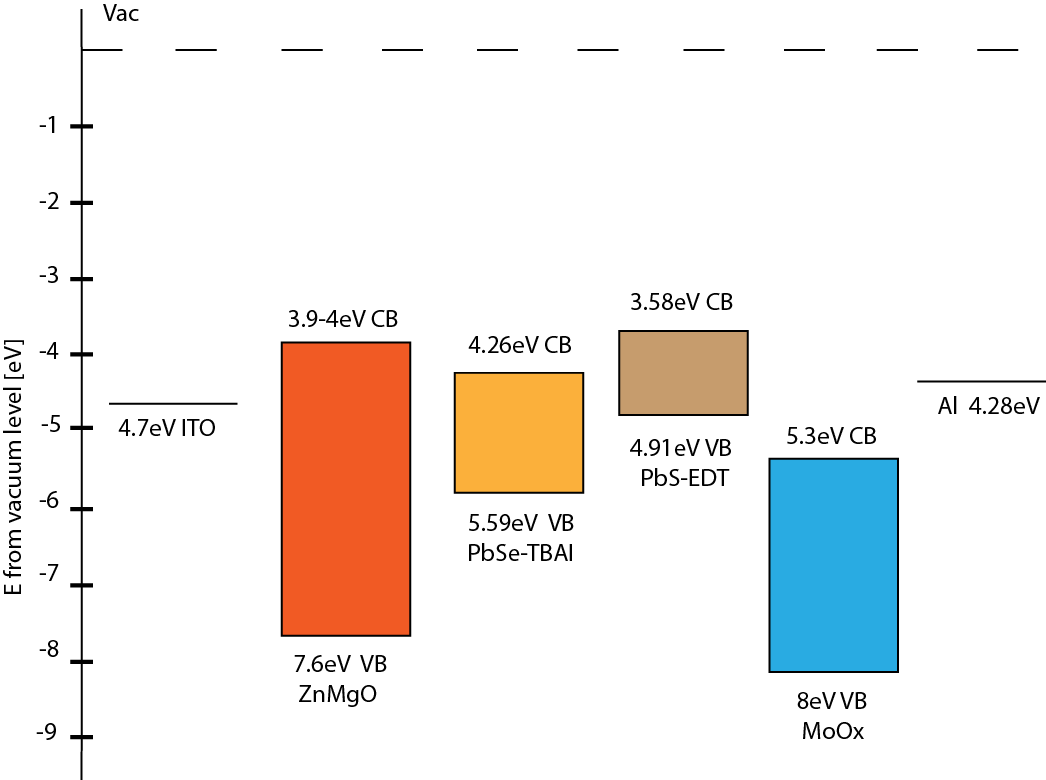
\includegraphics[width=0.6\textwidth]{ch5/STRUCTURE}
\caption{Energy structure of the first PbS-based QDSC}
\label{fig:1stEnergy}
\end{figure}

\subsubsection{Device fabrication}
\noindent The support for a whole device was ITO-coated glass substrate that was cleaned with strong solvents and drained ultrasonically. After that a double layer of MgO was created by using a spin-coater and after annealing PbS QDs were fabricated using spin-coating as well. It is important to denote, that it was possible to create a multi-deposition layers of QDs, which means the structure isn’t eluted from the ground. The layers were successfully dried in vacuum. After that, a MoOx firm has been added for creating inside trapping states and 
with sputtering process Al contacts were created on the device. As many heavy-metal QD semiconductors are toxic and degrade in air they must be also encapsulated in a stable polymer shell to avoid exposure. 
\begin{figure}
\center
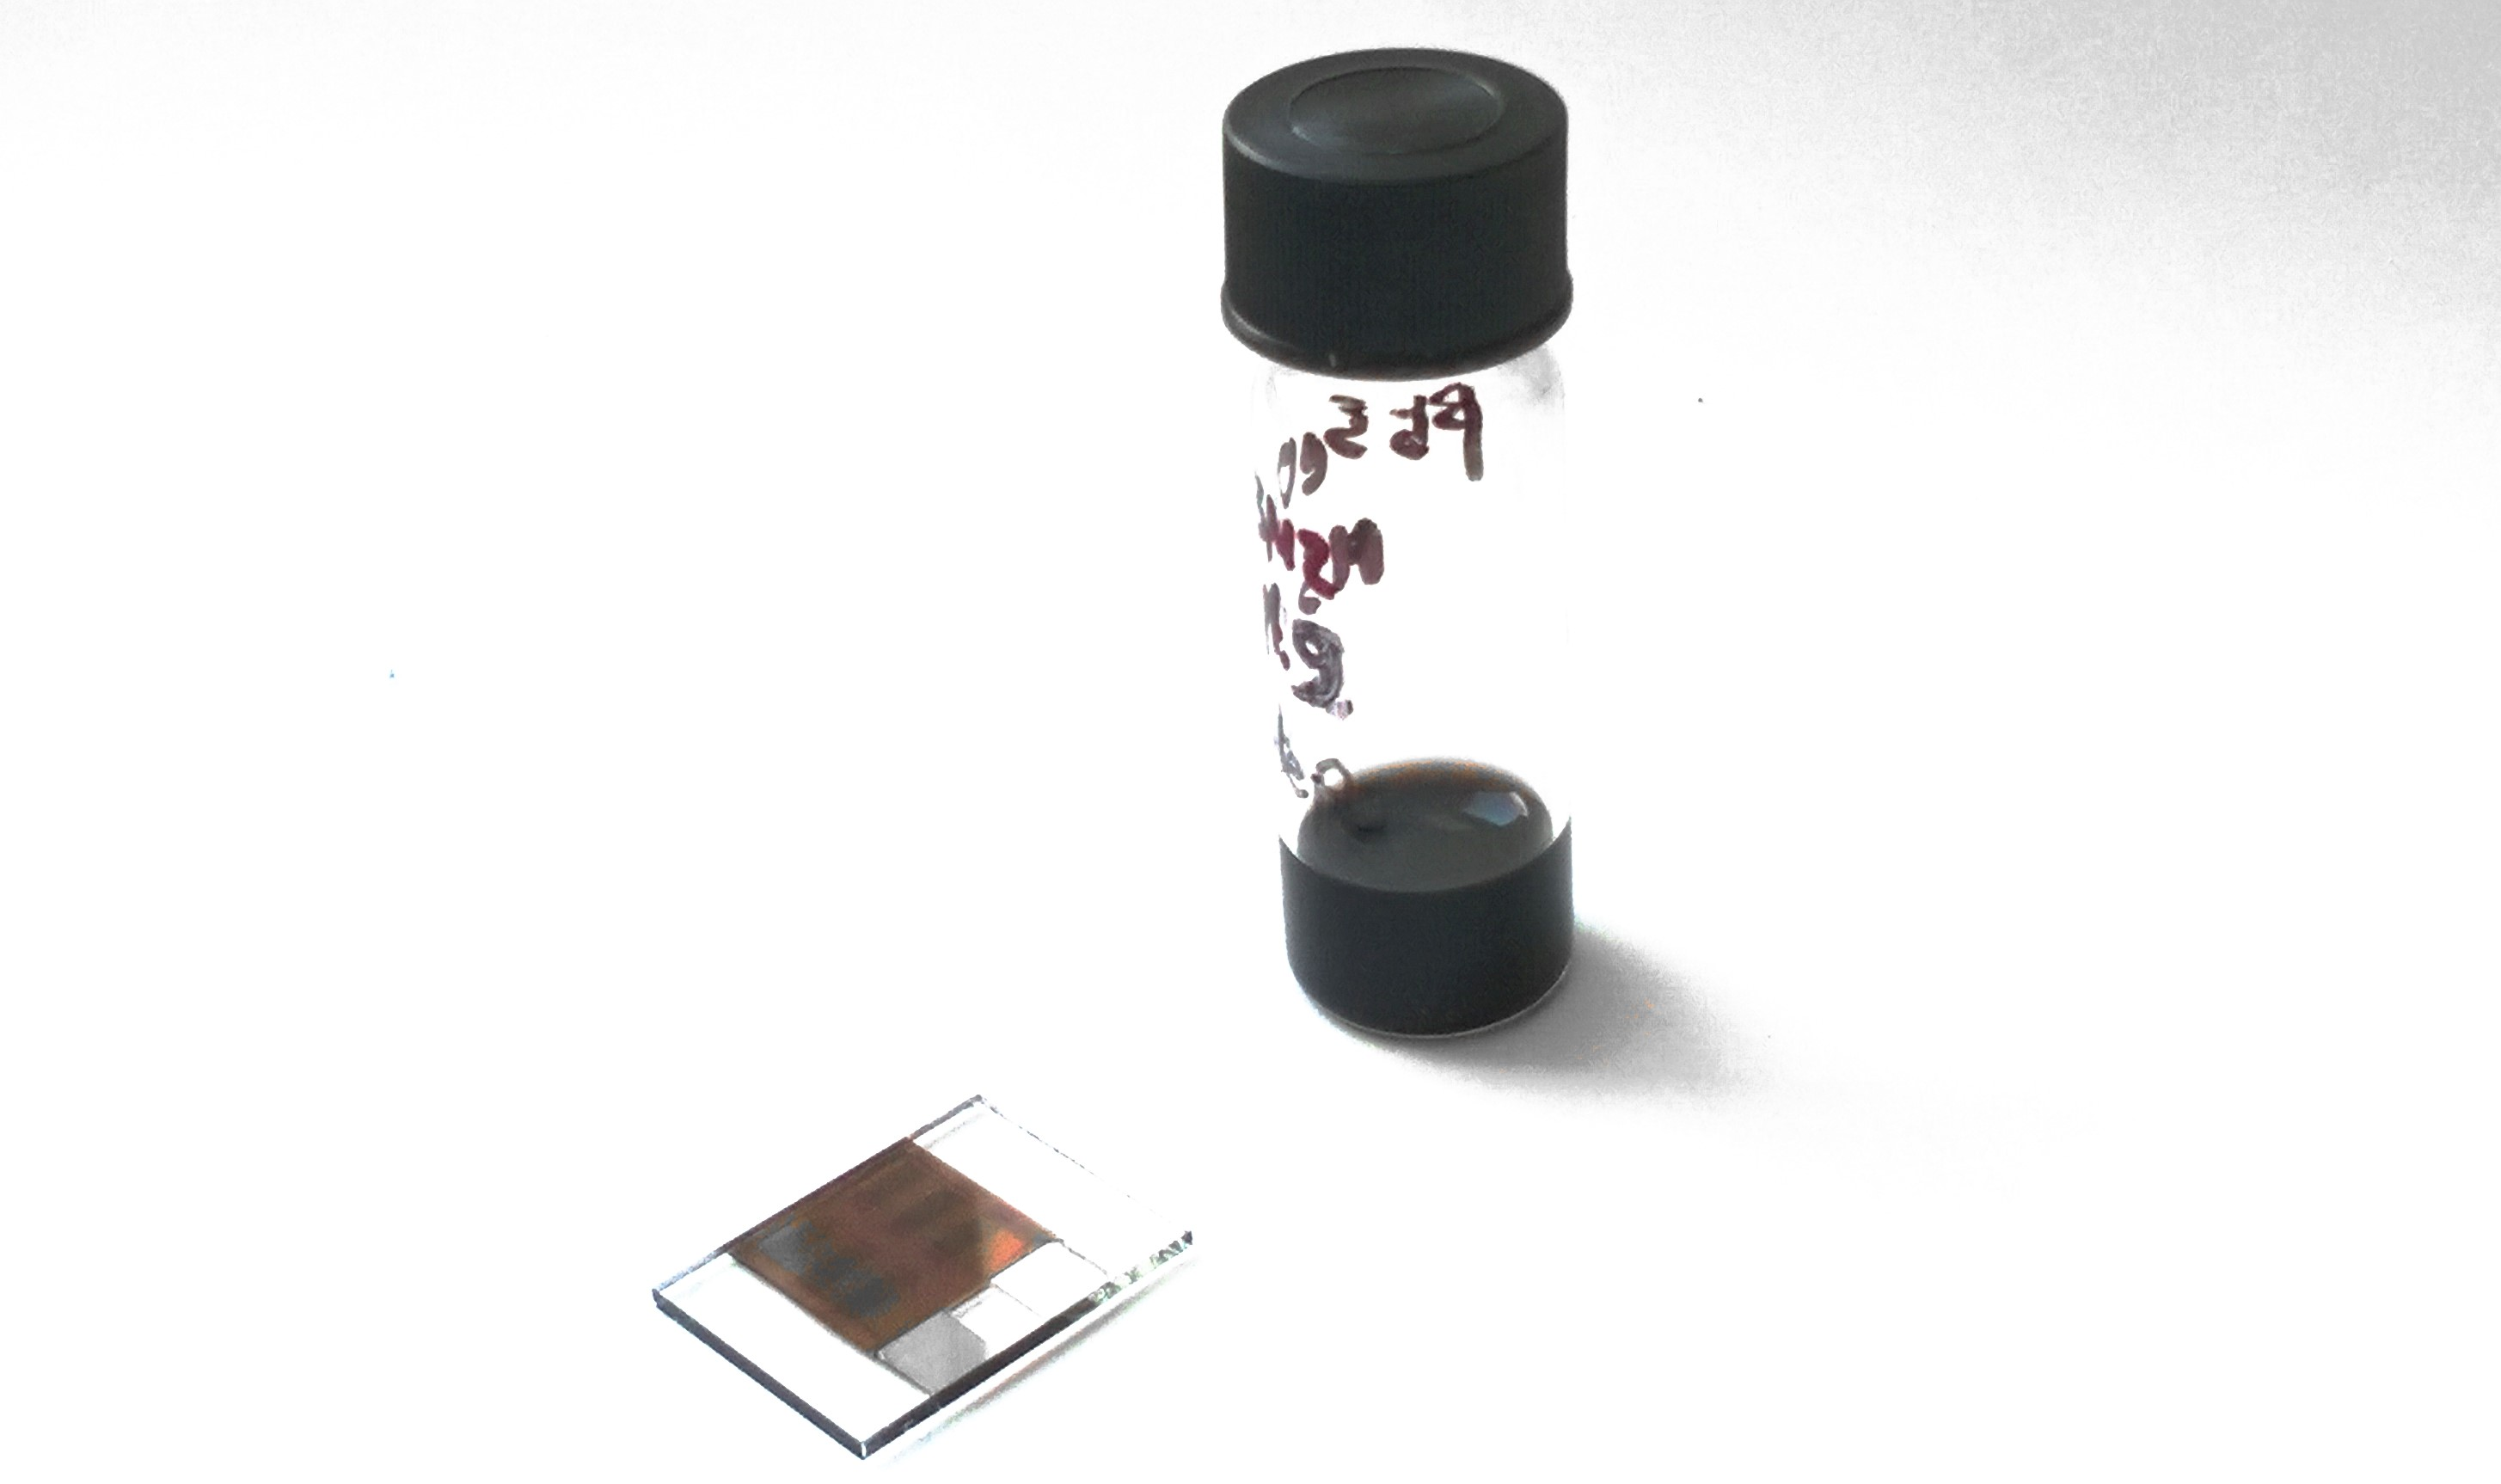
\includegraphics[width=0.6\textwidth]{ch5/IstSC}
\caption{First device and PbS Quantum-Dots produced in our lab}
\end{figure}

\subsubsection{Results}
From the following calculations we were able to compare both of the solar cells to distinguish what shall be definitely improved to achieve better effects. 
\begin{wrapfigure}{l}{0.451\textwidth}
\center
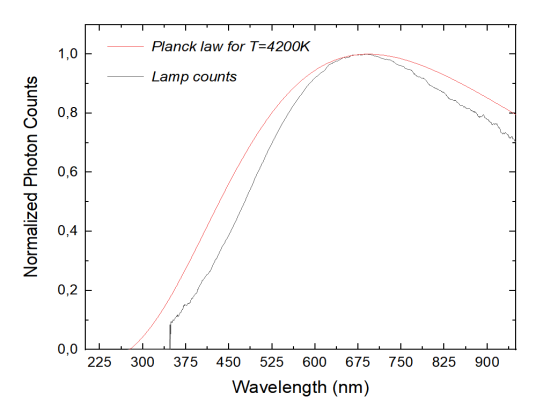
\includegraphics[width=0.45\textwidth]{ch5/bb1stco}
\caption{Comparison of Black Body photon counts and that of our light source}
\end{wrapfigure}
Standard photovoltaic measurements were provided to create IV both IV characteristics. However, it has to be denoted that neither were the surfaces of both devices the same, nor were the lengths from the light source. 

\noindent Therefore a certain calculations and assumptions were made. From the
photo-diode detector which were illuminated from the light source from
\(h_{d} = 400mm\) we calculate the \(P_{d}\)-power on the detector. We know that the photo-diode responsivity: \\ \\ \\ \\ 

\begin{equation}
R_{\lambda} = \frac{I_{p}}{P} = \frac{I_{p}}{r_{p} \cdot \frac{\text{hc}}{\lambda}}
\end{equation}


\noindent where \(I_{p}\) is a photo-current output, and P is a ratio of radiant
energy incident on the photodiode, which directly enables to calculate
\(r_{p} -\) photon flux(number of photons/sec). We also define quantum
efficiency of a photodetector as:
\begin{equation}
\eta = \frac{r_{e}}{r_{p}}
\end{equation}


\noindent which is the number of light created electrons to number of incident
photons. That depends on wavelength through absorption coefficient,
thickness of layers etc. Therefore we can say that:

\begin{equation}
r_{e} = \eta r_{p} = \frac{\eta P}{\frac{hc}{\lambda}} \rightarrow I_{p} = \frac{e\eta P}{\frac{hc}{\lambda}}
\end{equation}


\noindent Therefore, responsivity may be written as:

\begin{equation}
R_{\lambda} = \frac{e\eta P}{hc}
\end{equation}


\noindent According to those calculations we now see that from:
\begin{equation}
J_{sc} = e\int_{\lambda}^{}{\Phi_{p}(\lambda ) \cdot \eta (\lambda) d \lambda }
\end{equation}

\noindent \(\Phi_{p} -\) is a photon flux now, for the sake of new calculations to
distinguish the difference of photon counts and J­\textsubscript{sc} is
a short-circuit current. From that of above we now can see that:
\begin{equation}
J_{\text{sc}} = \int_{\lambda}^{}{\Phi_{p}\left( \lambda \right) \cdot R_{\lambda } \cdot \frac{\text{hc}}{\lambda }d\lambda } \rightarrow
\end{equation}

\begin{equation}
J_{\text{sc}}^{\text{rel}} = \int_{\lambda}^{}{\Phi_{p}^{\text{norm}}\left( \lambda \right) \cdot R_{\lambda} \cdot \frac{\text{hc}}{\lambda}d\lambda }
\end{equation}


\noindent where we have used relative value for short-circuit thanks to using a
normalised values because of the fact that detector isn't ideal and that
we can calculate the number of incident photons by simply using:
\begin{equation}
N_{p} = \frac{J_{sc}}{J_{sc}^{rel}}
\end{equation}

\noindent From now we can clearly say that:
\begin{equation}
P_{d} = \int_{\lambda}^{}{\Phi_{p}^{\text{norm}}\left( \lambda \right) \cdot N_{p} \cdot \frac{\text{hc}}{\lambda}d \lambda }
\end{equation}

\begin{figure}[H]
\center
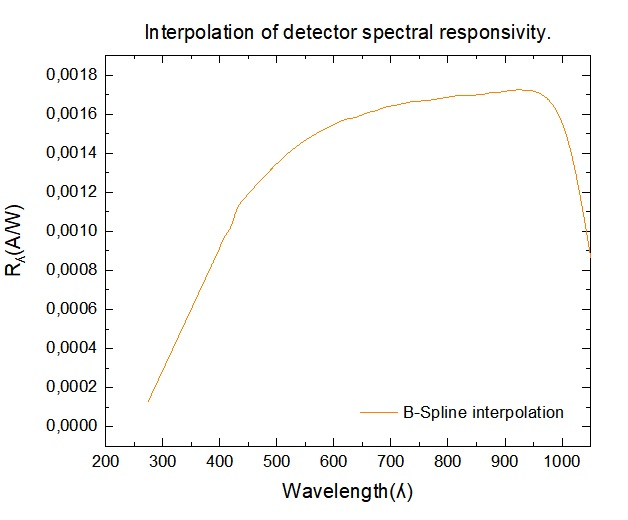
\includegraphics[width=0.8\textwidth]{ch5/GHZOPT}
\caption{Original data from Gigahertz Optik Gmbh}
\end{figure}

\noindent From integration and minding that
\(J_{\text{sc}} = 3,5 \cdot 10^{- 4}\text{mA\ }\)we achieved that:

\[N_{p} \approx 1,4 \cdot 10^{21}\]

\[P_{d} \approx 2,71 \cdot 10^{-4} \left( W \right)\ \]

\noindent The calculations are very roughly approximated and are just a
presentation of methods used, mainly due to the fact that the full
spectral characteristics weren't absolutely known. We can now estimate
\(P_{\text{density}} \approx \frac{P}{\Omega},\) where \(\Omega\) is a
solid angle. Therefore in our case from the information from \ref{tab:1stparam} we can calculate PCEs of both
photovoltaic devices by using:
\begin{figure}[b]
	\centering
	\begin{subfigure}[b]{0.49\textwidth}
	\centering
	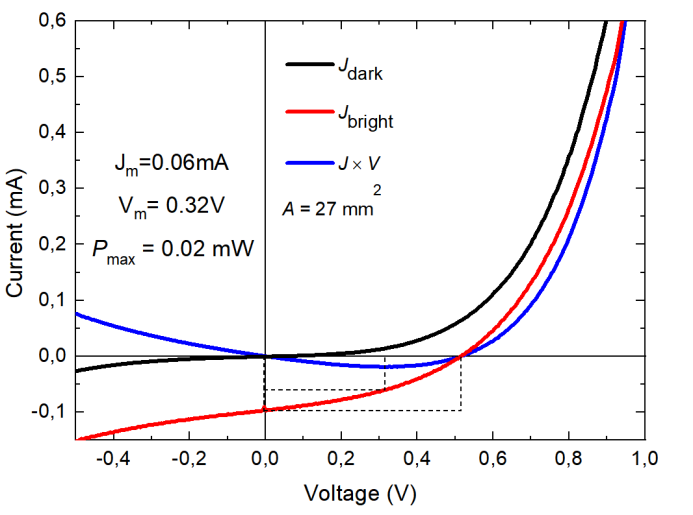
\includegraphics[width=0.93\textwidth]{ch5/istQDiv}
	\caption{QDSC}
	\end{subfigure}
	\hfill
	\begin{subfigure}[b]{0.49\textwidth}
	\centering
	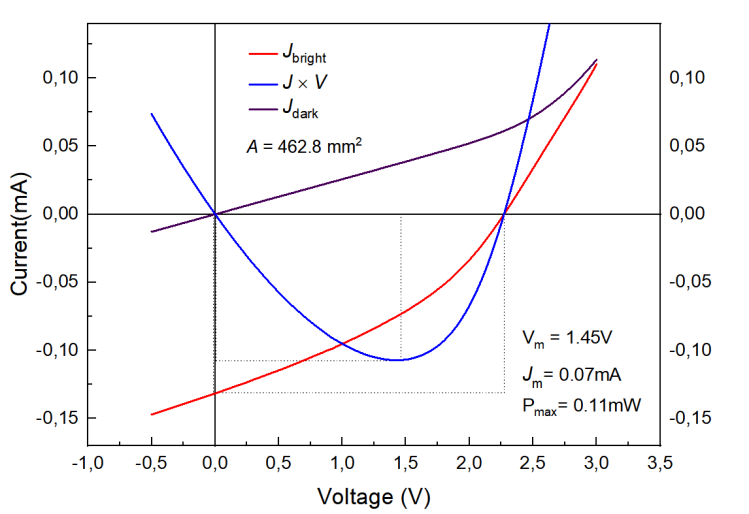
\includegraphics[width=\textwidth]{ch5/istVIMiv}
	\caption{Commercial solar cell}{}
	\end{subfigure}
	\caption{IV characteristics for QDSC and commercial cell }
\end{figure}

\begin{table}[h]
\centering
\begin{tabular}{|c |c | c | c |}
\hline
& Detector & QDSC & Commercial Cell\\
\hline
Length from light source{[}mm{]} & 400 & 75 & 603\\
\hline
Surface{[}mm\textsuperscript{2}{]} & 36,32 & 27 & 462,8\\
\hline
Solid angle{[}sr{]} & 2,27E-04 & 4,80E-03 & 1,27E-03\\
\hline
Incident Power {[}W{]} & 2,72E-01 & 2,02E-03 & 3,47E-03\\
\hline
\end{tabular}
\caption{Parameters of tested solar cells}
\label{tab:1stparam}
\end{table}

\begin{equation}
PCE = \frac{V_{m}J_{m}}{P_{\text{in}}}
\end{equation}

\begin{table}[h]
\centering
\begin{tabular}{|c |c |c | c | c|}
\hline
& V\textsubscript{m}{[}V{]} & I\textsubscript{m}{[}A{]} &P\textsubscript{in}{[}W{]} & PCE\\
\hline
QDSC & 0,32 & 6E-05 & 5,75E-03 & 0,33$\%$\\
\hline
Commercial Cell & 1,45 & 7E-05 & 1,53E-03 & 6,65$\%$\\
\hline
\end{tabular}
\caption{PCEs of photovoltaic devices}
\label{tab:1stPCE}
\end{table}
\noindent Provided that producer of the Commercial Cell provides similar PCE
compared to the given in \ref{tab:1stPCE} and the efficiency of our light
source is aimed to be close to 10\%, and therefore its power is 150W we
get circa 15W of light which we get by multiplying the power on the
detector by a factor of $4\pi /\Omega $ , where $\Omega$ is the solid angle for the
detector. This means that our, certainly course, calculations show
reasonable results from which we can definitely draw some conclusions.

\subsubsection{Conclusions and future prospects}

As we can clearly see, the PCE of QDSC made is small compared to the
current world efficiencies \cite{Kamat2018}. This can be caused by numerous reasons.
Working with colloidal quantum dots is always connected with the careful
arrangements of various parameters. The slightest change of just one may
provide a drastic change in the final result. Therefore we may conclude
that the reason of such an efficiency is mostly challenged by the
optimal choice of the layer width, quick degradation of QDs in the
presence of air or physical defects on the device structure. The large
leakage current may suggest that there are many defects inside the
device structure which simply create traps for moving electrons.
Nevertheless, the prospect of creating competitive QDSC is definitely in
our reach. For example, we can see that V\textsubscript{oc} is really
large for device with such a small surface. Now, we have to deal with
the improvement of our device. Optimization of the layer width and
enlarging of CQDs stability will be the first things to do, but
certainly not last. After testing those aspects, we may check if there
is another way to exchange ligands in CQDs, which may provide major
improvement in mobility, if there is growth of efficiency when changing
or adding another transport layer in the device structure or if layer
homogeneity can be further increased to stay comprehensive and
competitive.










\chapter{Results}


\chapter{Future possibilities}





\addcontentsline{toc}{chapter}{BIBLIOGRAPHY}
\printbibliography

\end{document}